%! TEX root = LaTeX_tips.tex

% Authors: Riccardo Milani, X12

% Acknowledgments: Cl\'ement Colas, Ga\"etan Mangeon, Germain Davy

\documentclass[a4paper,12pt,%
              final%
              %draft%
              ]{article}

\usepackage[english]{babel}
\usepackage[utf8]{inputenc}
\usepackage[T1]{fontenc}
%\usepackage{lmodern}

\usepackage[top=3cm, bottom=3cm, left=2cm, right=2cm]{geometry}

\usepackage{xcolor}
\definecolor{BlueX}{RGB}{0,62,92}
\def\maincolor{BlueX}

\usepackage{verbatim}
\usepackage{fancyvrb}

\usepackage{amsmath,amssymb,amsfonts,mathtools,amsthm}
\usepackage{empheq}

\usepackage[pdfpagelabels]{hyperref}

\usepackage{lipsum}

\usepackage{paralist}

\usepackage{enumitem}
\setlist[itemize]{topsep=0pt,noitemsep}

\usepackage{xspace}

\usepackage{tikz}
\usetikzlibrary{trees}
\usepackage{forest}

\usepackage{titlesec} % Modify the style of the sections, chapters...
\titleformat{\section} %command
    %[display] %shape
    {\color{\maincolor}\Large\bfseries\itshape} %format
    {\color{\maincolor}\Large\bfseries\itshape\thesection~-} %label
    {1ex} %sep
    {} %before-code
    %{} %after-code
\titleformat{\subsection} %command
    %[display] %shape
    {\color{\maincolor}\large\bfseries} %format
    {\color{\maincolor}\large\bfseries\thesubsection~-} %label
    {.5ex} %sep
    {} %before-code
    %{} %after-code

\parindent=0pt
\setlength{\parskip}{2ex}

\title{\color{\maincolor}\Huge\bfseries\scshape Random (and possibly useful) \LaTeX~tips}
\author{\vspace{-7ex}}
\date{\vspace{-7ex}}
\addto\captionsenglish{% Needed if babel is used. It is needed for every language that will be used.
  \renewcommand{\abstractname}{\vspace*{-\baselineskip}}%
}
%
\begin{document}

\maketitle
%\begin{center}
%{\color{\maincolor}\Huge\bfseries\scshape%
  %Random (and possibly useful) \LaTeX~tips}
%\end{center}
\vspace*{-2,5cm}

\begin{abstract}
\parindent=0pt
\setlength{\parskip}{2pt}
\noindent We collect here some \LaTeX~tricks that we used (do not ask why) and that we found useful. We hope that this list could save some Googlin', roaming around StackExchange and, most importantly, time to other people who may happen to need the same things.

There is no particular structure or whatsoever. We identified some major themes and then simply put an itemize in there. A brief ToC is given here below.

We try to give the snippet of the solution, hopefully commented, and an example: please copy them, and play around with them in order to make them suit your desires! If a loading of a package is required, you'll often see \verb|%...| or alike, usually meaning that what comes before it, goes in the preamble, what comes next into the document. Sometimes, when we were too lazy and we found it pretty clear, a link to an on-line solution is given. You'll find words in \texttt{< >}, that means that it is something that you have to / can choose. When discussing a package, we often provide the link to the PDF of the user manual: this might change and not be accessible anymore, if that happens, just google "ctan <name\_of\_the\_package>" and open the related CTAN address, and please, modify the link in this document, or, at least, report the issue.

If you liked and you have some cool tricks that you want to share in order to make other people's lives easier, do not hesitate to contribute: along with this file, you should have received its \href{run:./LaTeX_tips.tex}{source code} (of course we wrote it in \LaTeX, what do you expect?!); if not, ask for it (there are some tricks inside it, too!).

Happy \LaTeX ing! And remember: {\itshape Sharing is caring!}
\end{abstract}
%\clearpage

\tableofcontents
%\clearpage
%%%%%%%%%%%%%%%%%%%%%%%%%%%%%%%%%%%%%%%%%%%%%%%%%%%%%%%%%%%%%%%%%%%%%%%%%%%%%%%%
%%%                   SECTION: SECTIONING
%%%%%%%%%%%%%%%%%%%%%%%%%%%%%%%%%%%%%%%%%%%%%%%%%%%%%%%%%%%%%%%%%%%%%%%%%%%%%%%%
\section{Structure, Sectioning \& General Layout}
\label{sec:Sectioning}
\begin{itemize}
  \item Manage a big, multi-file project: \verb|\input| vs. \verb|\include|, \verb|\includeonly|, packages \href{https://ctan.mc1.root.project-creative.net/macros/latex/contrib/import/import.pdf}{\texttt{import}} and \href{http://mirror.ibcp.fr/pub/CTAN/macros/latex/contrib/subfiles/subfiles.pdf}{\texttt{subfiles}}; have a look \href{https://en.wikibooks.org/wiki/LaTeX/Modular_Documents}{here}.
  \item General introduction to a structure of a document: \href{https://en.wikibooks.org/wiki/LaTeX/Document_Structure}{here}
    \begin{itemize}
      \item The \texttt{book} class has a special \href{https://en.wikibooks.org/wiki/LaTeX/Document_Structure#Book_structure}{structure}: \verb|\frontmatter|, \verb|\mainmatter|, \verb|\appendix|, \verb|\backmatter|.
    \end{itemize}
  \item Modify first indentation: \verb|\parindent=<len>|
  \item Customize titling style: package \href{http://mirrors.ircam.fr/pub/CTAN/macros/latex/contrib/titlesec/titlesec.pdf}{\texttt{titlesec}}; an examples
\begin{Verbatim}[samepage=true]
\titleformat{\section} % Command: chapter, subsection...
    %[display] % Shape - Optional
    {\color{\maincolor}\Large\bfseries\itshape} % Format
    {\color{\maincolor}\Large\bfseries\itshape\thesection~-} % Label
    {1ex} % Separation
    {}    % Before-code
    %{}   % After-code - Optional
\end{Verbatim}
  \item Indent first line after section. Depending on (the typographic rules of) the chosen language, the first line after a non-centered titled \emph{section} may not be indented. If you would like to indent it anyway, just load \verb|\usepackage{indentfirst}|.
  \item Indent a \emph{whole} paragraph: have a look \href{https://tex.stackexchange.com/questions/35933/indenting-a-whole-paragraph}{here}.
  \item Numbering and ToC depth (how many levels are printed):
    \begin{itemize}
      \item \verb|\seccounter{secnumdepth}<n>|: define up to which level of sectioning titles are numbered.
      \item \verb|\setcounter{tocdepth}{<n>}| (mind that you can change the numbered level with \verb|\setcounter{secnumdepth}{<n>}| so that they are included in the ToC, but it is not exactly the same thing, as it is explained \href{https://tex.stackexchange.com/questions/17877/how-to-show-subsubsections-and-paragraphs-in-toc/17879#17879}{here}).
      \item Selectively change the depth: have a look \href{https://en.wikibooks.org/wiki/LaTeX/Document_Structure#Table_of_contents}{here} or \href{https://tex.stackexchange.com/questions/59091/setcountertocdepth}{here}.
    \end{itemize}
  \item Lengths and skips: \href{https://tex.stackexchange.com/questions/41476/lengths-and-when-to-use-them}{here}.
\end{itemize}

%%%%%%%%%%%%%%%%%%%%%%%%%%%%%%%%%%%%%%%%%%%%%%%%%%%%%%%%%%%%%%%%%%%%%%%%%%%%%%%%
%%%                   SECTION: FONT & APPEARANCE
%%%%%%%%%%%%%%%%%%%%%%%%%%%%%%%%%%%%%%%%%%%%%%%%%%%%%%%%%%%%%%%%%%%%%%%%%%%%%%%%
\section{Font, Appearance \& Spacing}
\label{sec:font}
\begin{itemize}
  \item \href{https://en.wikibooks.org/wiki/LaTeX/Fonts}{A general intro};
  \item Be advised that \verb|\emph{.}| does not not necessarily means italic. You might modify it as reported \href{https://tex.stackexchange.com/questions/315058/change-the-behaviour-of-emph-per-environment}{here} or \href{https://tex.stackexchange.com/questions/315058/change-the-behaviour-of-emph-per-environment}{here};
  \item Change default font style: \verb|\renewcommand{\familydefault}{<family>}| where \texttt{family} may be chosen in: \verb|\rmdefault| {roman family font}, \verb|\sfdefault| (sans serif family font), or \verb|\ttdefault| (teletype font family)
  \item Font sizes: see \autoref{tab:sizes}. Note that the last two \verb|\Tiny| and \verb|\TYNY| are available only with \texttt{beamer}.
  \item Font styles: see \autoref{tab:styles}.
  \item \LaTeX~lengths: have a look \href{https://www.overleaf.com/learn/latex/Lengths_in_LaTeX}{here} or even \href{https://en.wikibooks.org/wiki/LaTeX/Lengths}{there}.
  \item Spacing:
  \begin{itemize}
    \item \verb|\vspace{<length>}| (resp. \verb|\hspace{<length>}|) tells \LaTeX~to leave a vertical (resp. horizontal) space. Its starred version \verb|\vspace*{<len>}| forces it when you are close to the top/bottom of the page.
    \item For leaving one-time space between two lines, use \verb|\smallskip|, \verb|\medskip| or \verb|\bigskip| (which are equivalent to e.g. \verb|\vspace{\smallskipamount}|).
    \item \verb!\small|med|bigbreak!: as above but suggests to \LaTeX~that it would be a good place for a pagebreak if necessary.
    \item When forcing a newline, a custom vertical space may be added: \verb|The end\\[3cm]|.
    \item Fill the line/page: \verb!\hfill!, \verb!\vfill!. Might be useful: for lines \verb|\dotfill|, \verb|\hrulefill|.
  \end{itemize}
  \item Change the space after paragraph: \verb|\setlegth{\parskip}{<len>}|
  \item Spacing after a command
    \begin{itemize}
      \item Use a user-defined command and empty brackets as suggested \href{https://tex.stackexchange.com/questions/31091/space-after-latex-commands}{here}. Examples:
\begin{verbatim}
\newcommand{\cmd}{command}
A space after my \cmd{} here. There shouldn't be one after my \cmd{}.
\end{verbatim}
\newcommand{\cmd}{command}
      gives:\\
      A space after my \cmd{} here. There shouldn't be one after my \cmd{}.
      \item Use package \texttt{xspace} as explained \href{https://tex.stackexchange.com/questions/362046/insert-a-space-after-a-command-vs-vs-space}{here}.
\begin{verbatim}
\usepackage{xspace}
\newcommand{\cmd}{command\xspace}
A space after my \cmd here. There shouldn't be one after my \cmd.
\end{verbatim}
\newcommand{\cmdd}{command\xspace}
      A space after my \cmdd{} here. There shouldn't be one after my \cmdd{}.
    \end{itemize}
  \item Special and Accented characters: \href{https://en.wikibooks.org/wiki/LaTeX/Special_Characters#Escaped_codes}{here} (the link is useful for other symbols as well).
  \item Underline styles. The package \href{https://mirrors.chevalier.io/CTAN/macros/latex/contrib/ulem/ulem.pdf}{\texttt{ulem}} provides several underline styles (double, wavy, strike-out\ldots).
    \begin{itemize}
      \item It redefines the \verb|\emph{[...]}| command to underlined (instead of italic). Add option \texttt{normalem} to avoid that: \verb|\usepackage[normalem]{ulem}|.
    \end{itemize}
\end{itemize}
\begin{table}
  \centering
  \caption{Font sizes}
  \label{tab:sizes}
  \begin{tabular}{lc}
    \verb|\Huge| & {\Huge The quick brown fox\par}\\
    \verb|\huge| & {\huge The quick brown fox\par}\\
    \verb|\LARGE| & {\LARGE The quick brown fox\par}\\
    \verb|\Large| & {\Large The quick brown fox\par}\\
    \verb|\large| & {\large The quick brown fox\par}\\
    \verb|\normalsize| & {\normalsize The quick brown fox\par}\\
    \verb|\small| & {\small The quick brown fox\par}\\
    \verb|\footnotesize| & {\footnotesize The quick brown fox\par}\\
    \verb|\scriptsize| & {\scriptsize The quick brown fox\par}\\
    \verb|\tiny| & {\tiny The quick brown fox\par} \\
    \verb|\Tiny| & [\texttt{beamer} only] \\
    \verb|\TINY| & [\texttt{beamer} only] \\
  \end{tabular}
\end{table}
\begin{table}
  \centering
  \caption{Font styles}
  \label{tab:styles}
  \begin{tabular}{lll}
    Command & Switch & Output \\
    \hline
    \verb|\textnormal{...}| & \verb|{\normalfont ...}| & \textnormal{document font family}\\
    \verb|\emph{...}| & \verb|{\em ...}| & \emph{emphasis}\\
    \verb|\textrm{...}| & \verb|{\rmfamily ...}| & \textrm{roman font family}\\
    \verb|\textsf{...}| & \verb|{\sffamily ...}| & \textsf{sans serif font family}\\
    \verb|\texttt{...}| & \verb|{\ttfamily ...}| & \texttt{teletype font family}\\
    \verb|\textup{...}| & \verb|{\upshape ...}| & \textup{upright shape}\\
    \verb|\textit{...}| & \verb|{\itshape ...}| & \textit{italic shape}\\
    \verb|\textsl{...}| & \verb|{\slshape ...}| & \textsl{slanted shape}\\
    \verb|\textsc{...}| & \verb|{\scshape ...}| & \textsc{Small Capitals}\\
    \verb|\textbf{...}| & \verb|{\bfseries ...}| & \textbf{bold}\\
    \verb|\textmd{...}| & \verb|{\mdseries ...}| & \textmd{medium weight, normal}\\
    %\verb|\textlf{...}| & \verb|{\lfseries ...}| & \textlf{light}\\
    \verb|\uppercase{...}| &  & \uppercase{All caps}\\
    \verb|\lowercase{...}| &  & \lowercase{LOWER CAPS}
  \end{tabular}
\end{table}

%%%%%%%%%%%%%%%%%%%%%%%%%%%%%%%%%%%%%%%%%%%%%%%%%%%%%%%%%%%%%%%%%%%%%%%%%%%%%%%%
%%%                   SECTION: LANGUAGES
%%%%%%%%%%%%%%%%%%%%%%%%%%%%%%%%%%%%%%%%%%%%%%%%%%%%%%%%%%%%%%%%%%%%%%%%%%%%%%%%
\section{Languages}
\label{sec:languages}
Sometimes, especially in a thesis, one may have to use different languages, possibly with different typesetting styles (e.g. white-space before semicolon in French not in English). \href{https://en.wikibooks.org/wiki/LaTeX/Internationalization}{Here}, one can find an article about the internalization with pieces of advice and examples. When juggling more than one languages, the \texttt{babel} package comes in hand.
\begin{itemize}
  \item Load the \texttt{babel} package with the languages you want to use as options. The order is important since the last one is considered as default one:
\begin{verbatim}
\usepackage[<secondary_language>,<main_language>]{babel}
\end{verbatim}
  Thus, if one want to use French and English with the latter as default one would write \verb|\usepackage[french,english]{babel}|
  Even simpler, use the key \texttt{main}:
\begin{verbatim}
 \usepackage[french,main=english]{babel}
\end{verbatim}
  \item When a paragraph should be typeset / written in French, one should just switches the language with the help of the \texttt{otherlanguage} environment (an example \href{https://tex.stackexchange.com/questions/20987/changing-babel-package-inside-a-single-chapter}{here}):
\begin{Verbatim}[samepage=true]
[English typesetting]
\begin{otherlanguage}{french}
[French typesetting]
\end{otherlanguage}
[English typesetting]
\end{Verbatim}
  \item For some languages (e.g. Italian) \texttt{babel} changes autonomously caption names (figure, table,\ldots) and stuff (table of contents\ldots). With \texttt{french} (and similar) this does not happen for everything, hence one may want to rename manually the captions. For instance, one can use: \verb|\addto\captionsfrench{\def\tablename{Tableau}}|.
\end{itemize}

%%%%%%%%%%%%%%%%%%%%%%%%%%%%%%%%%%%%%%%%%%%%%%%%%%%%%%%%%%%%%%%%%%%%%%%%%%%%%%%%
%%%                   SECTION: ITEMIZE & Co.
%%%%%%%%%%%%%%%%%%%%%%%%%%%%%%%%%%%%%%%%%%%%%%%%%%%%%%%%%%%%%%%%%%%%%%%%%%%%%%%%
\section{Items \& Co.}
\label{sec:Items}
\begin{itemize}
  \item The \texttt{enumitem} \href{https://ctan.crest.fr/tex-archive/macros/latex/contrib/enumitem/enumitem.pdf}{package} enables more control on the \texttt{itemize} environment and alike.
    \begin{itemize}
      \item Usage
        \begin{itemize}
          \item Locally
\begin{verbatim}
\usepackage{enumitem}
% [...]
\begin{itemize}[<options>]
  \item [...]
\end{itemize}
\end{verbatim}
          \item Globally
\begin{verbatim}
\usepackage{enumitem}
\setlist[itemize]{<options>}
\end{verbatim}
        \end{itemize}
      \item Some options:
        \begin{itemize}
          \item No indent: \texttt{leftmargin=*};
          \item No separations between items: \texttt{noitemsep};
          \item No separations whatsoever: \texttt{nosep};
          \item Modify top spacing: \texttt{topsep=<len>};
          \item Modify the bullet: \texttt{label=<cmd>}. With a star, \texttt{label*=<cmd>}, \texttt{cmd} is repeated two times for sub-items, three for sub-sub-items, etc;
          \item Run a bit of code before/after the \texttt{itemize}: \texttt{before|after=<code>}
        \end{itemize}
      \item \verb|\setlist[<type>[,<depth>]]{<options>}|: in the preamble, and will set the global parameter for all the \texttt{type}-lists of depth \texttt{depth}. If \texttt{depth} is not given, the options are set to all (sub)-items. \texttt{type} may be \texttt{itemize,description,enumerate}...
\begin{verbatim}
\setlist[itemize]{%
  leftmargin=*} % No margin for all the items of itemize
\setlist[itemize,1]{%
  label=$\bullet$} % Items are circles
\setlist[itemize,2]{%
  label=$\triangleleft$} % Sub-items are left-facing triangles
\end{verbatim}
      \item Enumerations with a prefix: \href{https://tex.stackexchange.com/questions/37740/enumerate-with-properties}{here}. Just set the label as you wish as option:
\begin{verbatim}
\begin{enumerate}[label=\textbf{H\arabic*}]
  \item Property 1
  \item Property 2
\end{enumerate}
\end{verbatim}
      \item Enumerations starting from \texttt{<n>}: \verb|\begin{enumerate}[start=<n>]|
      \item \textbf{ATTENTION}: it may interfere with \texttt{beamer} and they may not work as expected if loaded together, see this \href{https://tex.stackexchange.com/questions/24371/does-enumitem-conflict-with-beamer-for-lists}{post} for two common problems.
      \item \textbf{ATTENTION}: it may cause some errors with the \texttt{enumerate} lists. In this case, load the option \texttt{shortlabels} and explicitly choose the type of item for the numeration
\begin{verbatim}
\usepackage[shortlabels]{enumitem}
% [...]
\begin{enumerate}[1.]
  \item One.
\end{enumerate}
\end{verbatim}
    \end{itemize}
  \item Inline lists: \href{https://mirrors.chevalier.io/CTAN/macros/latex/contrib/paralist/paralist.pdf}{\texttt{paralist}} package, and in particular its \texttt{inparaenum} environment.
    \begin{itemize}
      \item \textbf{ATTENTION}: load \texttt{paralist} \emph{before} \texttt{enumitem}.
      \item A similar result is obtained with the \texttt{inline} option of \texttt{enumitem}.
      \item \texttt{paralist} does not work properly with \texttt{beamer}.
    \end{itemize}
  \item Referencing and \texttt{itemize}
    \begin{itemize}
      \item There is no point (actually, no way neither) in referencing an item in an \texttt{itemize}: they all look the same, you can not tell them apart;
      \item \texttt{enumerate} items can be referenced by default with the \texttt{enumitem} package, an example \href{https://tex.stackexchange.com/questions/58713/ref-should-use-enumerate-label-name}{here};
      \item For \texttt{description} items:
\begin{Verbatim}[samepage=true]
\usepackage{enumitem, hyperref}
\makeatletter
\def\namedlabel#1#2{\begingroup
    #2%
    \def\@currentlabel{#2}%
    \phantomsection\label{#1}\endgroup
}
 %...
\begin{description}[style=multiline, labelwidth=1.5cm]
    \item[\namedlabel{itm:rule1}{Rule1}] What should I do?
    \item[\namedlabel{itm:rule2}{Rule2}] Reference to \ref{itm:Rule1}
\end{description}
\end{Verbatim}
    \end{itemize}
\end{itemize}

%%%%%%%%%%%%%%%%%%%%%%%%%%%%%%%%%%%%%%%%%%%%%%%%%%%%%%%%%%%%%%%%%%%%%%%%%%%%%%%%
%%%                   SECTION: TABLES
%%%%%%%%%%%%%%%%%%%%%%%%%%%%%%%%%%%%%%%%%%%%%%%%%%%%%%%%%%%%%%%%%%%%%%%%%%%%%%%%
\section{Tables}
\label{sec:Tables}
\begin{itemize}
  \item General info \href{https://en.wikibooks.org/wiki/LaTeX/Tables}{here}
  \item \verb|@{<ex>}|: put \texttt{<ex>} at the beginning of the following column on every row
\begin{verbatim}
\begin{tabular}{c@{:}c}
   Test  &  Test \\
  ReTest & ReTest
\end{tabular}
\end{verbatim}
\begin{itemize}
  \item \verb|@{}|: set the space between two columns to zero
\end{itemize}
    \item Fix a table width, you have to use at least once the column type \texttt{X}:
\begin{verbatim}
\usepackage{tabularx}
%...
\begin{tabularx}{<tablewidth>}{XX}
   Test  &  Test \\
  ReTest & ReTest
\end{tabularx}
\end{verbatim}
    \begin{itemize}
      \item Centered \texttt{X}-like column type: \href{https://tex.stackexchange.com/questions/89166/centering-in-tabularx-and-x-columns}{here}
\begin{verbatim}
\newcolumntype{Y}{>{\centering\arraybackslash}X}
\end{verbatim}
    \end{itemize}
  \item Merge cells: multirow \& multicolumn. Attention: multirow needs the \texttt{multirow} package
\begin{verbatim}
\multicolumn{<#cols to merge>}{<type>}{<content>}
\multirow{<#rows to merge>}{<width(or *)>}{<content>}
\end{verbatim}
    e.g.: \verb!\multicolumn{2}{c|}{Two columns in one}!
  \item Horizontal tables / landscape: use the environment \texttt{sidewaystable} (instead of \texttt{table}) from the package \texttt{rotating}. Other solution found \href{http://distrib-coffee.ipsl.jussieu.fr/pub/mirrors/ctan/macros/latex/required/tools/longtable.pdf}{here};
  \item Wider choice of row / column separators: see package \href{http://distrib-coffee.ipsl.jussieu.fr/pub/mirrors/ctan/macros/latex/required/tools/longtable.pdf}{\texttt{hhline}};
  \item Tables spanning more than one pages: use package \href{http://distrib-coffee.ipsl.jussieu.fr/pub/mirrors/ctan/macros/latex/required/tools/longtable.pdf}{\texttt{longtable}};
  \item Table and colors: the reference is \href{http://mirrors.ircam.fr/pub/CTAN/macros/latex/contrib/colortbl/colortbl.pdf}{\texttt{colortbl}} (which may be loaded by passing options \texttt{tables} to package \href{http://mirrors.standaloneinstaller.com/ctan/macros/latex/contrib/xcolor/xcolor.pdf}{\texttt{xcolor}}). Some tips \href{https://texblog.org/2011/04/19/highlight-table-rowscolumns-with-color}{here};
  \item For typesetting numerical data (but not necessarily), you may want to have a look at \texttt{pgfplotstable}, \autoref{sec:tikzpgf}.
  \item Colored and rounded tables (use of \texttt{TikZ}, \autoref{sec:tikzpgf}): some tips \href{https://tex.stackexchange.com/a/184075}{here} and example in \href{run:./ex_plot.tex}{\texttt{ex\_plot.tex}}.
\end{itemize}

%%%%%%%%%%%%%%%%%%%%%%%%%%%%%%%%%%%%%%%%%%%%%%%%%%%%%%%%%%%%%%%%%%%%%%%%%%%%%%%%
%%%                   SECTION: EQUATIONS
%%%%%%%%%%%%%%%%%%%%%%%%%%%%%%%%%%%%%%%%%%%%%%%%%%%%%%%%%%%%%%%%%%%%%%%%%%%%%%%%
\section{Math, Equations \& Theorems}
\label{sec:math}
\begin{itemize}
  \item Some good tips about equations and math mode in general can be found \href{https://en.wikibooks.org/wiki/LaTeX/Advanced_Mathematics}{here}. This short \href{http://www.math.hkbu.edu.hk/TeX/short-math-guide.pdf}{guide} is quite useful, as well. One can find good stuff \href{http://ctan.math.utah.edu/ctan/tex-archive/obsolete/info/math/voss/mathmode/Mathmode.pdf}{here}, too.
  \item Math symbols: basic ones can be found \href{http://web.ift.uib.no/Teori/KURS/WRK/TeX/symALL.html}{here} or \href{https://oeis.org/wiki/List_of_LaTeX_mathematical_symbols}{here}, otherwise, most modern IDE, such as \TeX Maker (cf. \autoref{sec:texmaker}) provides a list (anyhow, my advice: think in English).
  \item Usually, for every math environment there exists also its \texttt{-ed}-form to be used when math-mode is already activated. Mind:

\begin{minipage}[T]{.4\textwidth}
\begin{Verbatim}[frame=single]
[text-mode: on]
\begin{align}
  [math-mode: on]
  e^{i\pi}+1=0
\end{align}
[text-mode: on]
\end{Verbatim}
\end{minipage} \hspace*{2em}  vs.\hspace*{2em} \hfill %
\begin{minipage}[T]{.4\textwidth}
\begin{Verbatim}[frame=single]
[text-mode: on]
\begin{equation}
  [math-mode: on]
  \begin{aligned}
    e^{i\pi}+1=0
  \end{aligned}
\end{equation}
[text-mode: on]
\end{Verbatim}
\end{minipage}

  \item Matrices: have a look \href{http://www.sascha-frank.com/Faq/matrices.html}{here}. \texttt{matrix}, \texttt{pmatrix} (parentheses), \texttt{bmatrix} (brackets), \texttt{Bmatrix} (curly), \texttt{vmatrix} (vertical), \texttt{Vmatrix} (double vertical), \texttt{smallmatrix} (small inline matrix).
  \item Tagged equations: name instead of the usual number. Notice the unnumbered environment (in fact, you must not step the equation numbering)
\begin{verbatim}
\begin{equation*}
  e^{i\pi}+1=0 \label{eq:euler}\tag{Euler's}
\end{equation*}
\end{verbatim}
  \item Cross out term from equation, for instance if they vanish. Example:
\begin{verbatim}
\usepackage[makeroom]{cancel}
%[...]
\[ x + \cancel{y} = \]
\end{verbatim}
  \item Boxed equation. The simple one: \verb|\boxed{...}| from the \texttt{amsmath} package. The customizable one: the \texttt{empheq} environment from the \href{https://ctan.org/pkg/empheq}{\texttt{empheq}} package.
  \item Numbering and referencing inside a system: package \href{https://ctan.org/pkg/empheq}{\texttt{empheq}} is recommended.

        \begin{minipage}{.45\linewidth}
\begin{Verbatim}
\begin{empheq}%
  [left=\empheqlbrace]{align}
  aaa &= 0 \label{eq:emph_a} \\
  b &= 1 \label{eq:emph_b}
\end{empheq}
Reference \eqref{eq:emph_a}
and \eqref{eq:emph_b}.
\end{Verbatim}
        \end{minipage}\hspace{1cm} gives  \hspace{1cm}
        \begin{minipage}{.35\linewidth}
          \begin{empheq}%
            [left=\empheqlbrace]{align}
            aaa &= 0 \label{eq:emph_a} \\
            b &= 1 \label{eq:emph_b}
          \end{empheq}
          Reference \eqref{eq:emph_a} and \eqref{eq:emph_b}.
        \end{minipage}

  \item Sub-equations (get second numbering inside the same equation, for instance (1a), (1b),...): use the \texttt{subequations} environment from the package \texttt{amsmath}. Example:

    \begin{subequations}
      Euler's: \label{eq:one}
      \begin{align}
        e^{i\pi}+1=0\label{eq:one_a}\\
        \cos(\pi)+1=0\label{eq:one_b}
      \end{align}
    \end{subequations}
    \begin{itemize}
      \item ATTENTION: it does NOT switch to math mode, that means that we should call a math-mode-enabling environment inside it:
\begin{verbatim}
\begin{subequations}
  Euler's: \label{eq:one}
  \begin{align}
    e^{i\pi}+1=0 \label{eq:one_a}\\
    \cos(\pi)+1=0 \label{eq:one_b}
  \end{align}
\end{subequations}
\end{verbatim}
      \item In the example here above, unless you changed the default parameters, referencing \verb|eq:one| will give \eqref{eq:one}, \verb|eq:one_a| will give \eqref{eq:one_a} and \verb|eq:one_b| \eqref{eq:one_b}.
      \item Problems may arise when coupling it with brackets or \texttt{align}. Two workarounds are found \href{https://tex.stackexchange.com/questions/322087/bracket-in-subequations/323414#323414}{here} and \href{https://tex.stackexchange.com/questions/80134/nesting-subequations-within-align}{here}.
      \item Tags: look \href{https://tex.stackexchange.com/questions/284313/how-do-i-tag-a-subequations-environment-as-a-whole}{here}
    \end{itemize}
  \item About theorems:
    \begin{itemize}
      \item Define and use theorem style
\begin{Verbatim}[samepage=true]
 \newtheoremstyle{myRemark}% name of the style to be used
  {3pt}% space above the theorem. E.g.: 3pt
  {3pt}% space below the theorem. E.g.: 3pt
  {\itshape}% font to use in the body
  {}% measure of space to indent
  {\itshape\bfseries}% head font
  {.}% punctuation between head and body
  {.5em}% space after theorem head; " " = normal interword space
  {}% Manually specify head
\theoremstyle{myRemark} % Choose the style
%\newtheorem{env_name_to_call_in_tex}%
%     [continuing_the_same_numbering_as_this_thm_style]%
%     {Printed name}%
%     [second_numbering:reset_when_this_is_called]%
\newtheorem{rem}{Remark}[section] %Style = myRemark
\newtheorem{note}{Note}[section] %Style = myRemark

\theoremstyle{plain}
\newtheorem{thm}{Thm} %Style = plain
\end{Verbatim}
    \item Customize the title: \href{https://tex.stackexchange.com/questions/374359/how-to-place-the-definition-title-in-square-brackets-instead-of-paranthesis/374360}{here}
    \item Define names for referencing
\begin{verbatim}
\newcommand{\remautorefname}{Remark} % For autoref (hyperref)
%\crefname{<env>}{<singular>}{<plural>} % For cref (cleveref)
\crefname{rem}{Remark}{Remarks}
\end{verbatim}
    \end{itemize}
  \item All \texttt{align}-like environments have an intrinsic structure of \texttt{rlrl...} alignment, meaning that, the first column is right aligned, the second left aligned, and so on. You can tweak this by adding a void column.
\begin{verbatim}
\begin{aligned}
  a &= b &  text % text is right aligned
  c &= d &  text % text is right aligned
\end{aligned}
\begin{aligned}
  a &= b && text % text is left  aligned
  c &= d && text % text is left  aligned
\end{aligned}
\end{verbatim}
  \item Diagrams: \href{http://mirrors.ircam.fr/pub/CTAN/graphics/pgf/contrib/tikz-cd/tikz-cd-doc.pdf}{\texttt{tikz-cd}} might be useful.
%%%%%%%%%%%%%%%%%%%%%%%%%%%% LET THIS BE THE LAST
  \item Spacing: whitespaces are skipped in math mode, however, there are several ways to force them. See \autoref{tab:math_space}.
\end{itemize}
\begin{table}
  \centering
  \caption{Spacing in math mode}
  \label{tab:math_space}
  \begin{tabular}{lllc}
    \textvisiblespace & none         & \verb|$ a b c $| & $ a b c $ \\
    \verb|\,|         & thin space   & \verb|$ a\,b\,c $| & $ a\,b\,c $ \\
    \verb|\:|         & medium space & \verb|$ a\:b\:c $| & $ a\:b\:c $ \\
    \verb|\>|         & medium space & \verb|$ a\>b\>c $| & $ a\>b\>c $ \\
    \verb|\;|         & thick space  & \verb|$ a\;b\;c $| & $ a\;b\;c $ \\
    \verb|\|\textvisiblespace & thicker space  & \verb|$ a\ b\ c $| & $ a\ b\ c $ \\
    \verb|\quad|      & tab          & \verb|$ a\quad b\quad c $| & $ a\quad b\quad c $ \\
    \verb|\qquad|     & double tab   & \verb|$ a\qquad b\qquad c $| & $ a\qquad b\qquad c $ \\
  \end{tabular}
\end{table}


%%%%%%%%%%%%%%%%%%%%%%%%%%%%%%%%%%%%%%%%%%%%%%%%%%%%%%%%%%%%%%%%%%%%%%%%%%%%%%%%
%%%                   SECTION: BEAMER
%%%%%%%%%%%%%%%%%%%%%%%%%%%%%%%%%%%%%%%%%%%%%%%%%%%%%%%%%%%%%%%%%%%%%%%%%%%%%%%%
\section{Beamer}
\label{sec:Beamer}
Let's start by giving the full \href{http://mirrors.ircam.fr/pub/CTAN/macros/latex/contrib/beamer/doc/beameruserguide.pdf}{manual}, a quick \href{https://en.wikibooks.org/wiki/LaTeX/Presentations}{intro} and an appearance \href{http://www.cpt.univ-mrs.fr/~masson/latex/Beamer-appearance-cheat-sheet.pdf}{cheat sheet}.
\begin{itemize}
  \item Overlays, that is how to make something (dis)appear (e.g. \verb!\only!, \verb!\uncover!...): \href{https://openclassrooms.com/courses/creez-vos-diaporamas-en-latex-avec-beamer/les-overlays-1}{here} or also \href{https://www.texdev.net/2014/01/17/the-beamer-slide-overlay-concept/}{here}
    \begin{itemize}
      \item Syntax: \verb|\cmd<when>{...}| (mind that this time the angle brackets \verb|<.>| should really be there). Some examples, consider \verb|I'm am \only<when>{un}happy|, \texttt{un} is printed: \verb|\only<2>| on the second slide only, \verb|\only<-3>| on every slide up to slide 3, \verb|\only<2->| on slide 2 and following, \verb|\only<1-3,12>| on slides 1 to 3 and then on slide 12.
      \item \verb|\uncover<n>{What}|: the parameter will be invisible until slide n, but it will still be there hence it occupies some space. For instance, with \verb|\uncover<2>{Not} the beginning|, on slide one the line starts with a large whitespace which will only be filled on slide 2 (and on slide 2 only, otherwise we should have used \verb|\uncover<2->|) by \texttt{Not}
      \item \verb|<+>| increments the previous action:
\begin{verbatim}
\only<+>{3}\only<+>{2}\only<+>{1}\only<+>{Happy New Year!}
\end{verbatim}
        Hence, \verb|<+->| means "starting from the next and then on all the following":
\begin{verbatim}
Batmaaaan \only<+->{na}\only<+->{na}\only<+->{na}
\end{verbatim}
      \item In a series of \verb|<+->|, for example in an \verb|itemize|, the key \verb|.| (point) will repeat the previous overlay number, making the item appear at the same time as the previous one. An example taken from the second link:
\begin{Verbatim}[samepage=true]
  \begin{itemize}
    \item<+-> This is on the first and all following slides
    \item<.-> This is also on the first and all following slides
    \item<+-> This is on the second and all following slides
    \item<.-> This is also on the second and all following slides
  \end{itemize}
\end{Verbatim}
      \item \verb|\begin{overlayarea}{<width>}{<height>} ... \end{overlayarea}|
    \end{itemize}
  \item Numbering and appendix / backup slides:
    \begin{itemize}
      \item No numbering: \href{https://stackoverflow.com/questions/732902/ignoring-page-numbers-in-backup-slides}{here}
\begin{verbatim}
\begin{frame}[noframenumbering]{Title}
%  Lorem Ipsum
\end{frame}
\end{verbatim}
      \item New numbering only for the appendix: \href{https://tex.stackexchange.com/questions/70448/dont-count-backup-slides}{here}
\begin{verbatim}
\usepackage{appendixnumberbeamer}
%[...]
\appendix
\begin{frame}{First appendix frame}
%  Lorem Ipsum
\end{frame}
\end{verbatim}
      \item When compiling in handout mode, all the overlays are overwritten on a single slide. One can however control the handout slides with a similar syntax as the overlays. E.g. \verb!\only<1,3|handout:2>{Test}!: \verb|Test| will be printed on slides 1 and 3 when in presentation mode, but on slide 2 when in handout mode.
    \end{itemize}
  \item It has been seen \autoref{sec:Items} that \texttt{beamer} and \texttt{enumitem} may interfere, typically with this latter erasing the settings done by the former. Here how to restore the \texttt{beamer} bullets:
\begin{Verbatim}[samepage=true]
\setlist[itemize,1]{label=%
  \usebeamerfont*{itemize item}%
  \usebeamercolor[fg]{itemize item}%
  \usebeamertemplate{itemize item}}
\setlist[itemize,2]{label=%
  \usebeamerfont*{itemize subitem}%
  \usebeamercolor[fg]{itemize subitem}%
  \usebeamertemplate{itemize subitem}}
\end{Verbatim}
  \item At the beginning of each (sub)section add a frame with the table of contents and the current (sub)section highlighted: in you preamble
\begin{Verbatim}[samepage=true]
\AtBeginSection[] %
{ \begin{frame}<beamer>
\frametitle{Plan}
\tableofcontents[currentsection]
\end{frame} }

\AtBeginSubsection[] %
{ \begin{frame}<beamer>
\frametitle{Plan}
\tableofcontents[currentsubsection]
\end{frame} }
\end{Verbatim}
  \item Change the background: look \href{https://tex.stackexchange.com/questions/78464/background-image-in-beamer-slides}{here}.
  \item Include other slides in pdf: see the bullet about \texttt{pdfpages} in \autoref{sec:Miscellaneous}.
  \item Draft: just pass \texttt{draft} to \texttt{beamer}. If you want to only disable image loading, try: \verb|\PassOptionsToPackage{draft}{graphicx}| before \verb|\documentclass{...}| (\href{https://tex.stackexchange.com/questions/4370/disabling-included-pictures-in-beamer}{here}).
  \item \texttt{includeonly}-like (\autoref{sec:Sectioning}): define labels and filter as shown \href{https://tex.stackexchange.com/questions/4370/disabling-included-pictures-in-beamer}{here}
\begin{verbatim}
\includeonlyframes{foo}
%[...]
\begin{frame}[label=foo]
  First frame
\end{frame}
\begin{frame}[label=bar]
  Second frame, which will not be seen.
\end{frame}
\end{verbatim}
  \item Sections in ToC / navigation bar (list of sections in the header/footer): alternatives \href{https://tex.stackexchange.com/questions/66628/latex-beamer-frame-outside-sections}{here}.
  \item \texttt{beamer} introduces two new \emph{very} small font size: \verb|\Tiny| and \verb|\TINY| (\autoref{sec:font}).
  \item Option \texttt{allowframebreaks} passed to the \texttt{frame} environment allows to have a long content spanning more than one slides. This could be useful for bibliography for example that may require several slides
\begin{verbatim}
\begin{frame}[allowframebreaks]{A very long slide}
  [A very long conten]
\end{frame}
\end{verbatim}
    \begin{itemize}
      \item Insert a frame break with \verb|\pagebreak| (this applies both to presentation and handout mode), or \verb|\framebreak| (which is equivalent to \verb|\pagebreak<presentation>| and hence applies only to presentationmode)
    \end{itemize}
  \item It is possible to insert interactive buttons that allow one to, for instance, go to a slide and come back, go to the end/beginning, repeat a previous slide... The feature is possible via the \texttt{hyperref} package and it relies on \verb|\hyperlink{[..]}{<beamer_button>}|, \verb|\beamer<type>button{<name>}|... I know, not a very useful advice, but have a look at the manual or on StackExchange.
\end{itemize}

%%%%%%%%%%%%%%%%%%%%%%%%%%%%%%%%%%%%%%%%%%%%%%%%%%%%%%%%%%%%%%%%%%%%%%%%%%%%%%%%
%%%                   SECTION: GRAPHICS
%%%%%%%%%%%%%%%%%%%%%%%%%%%%%%%%%%%%%%%%%%%%%%%%%%%%%%%%%%%%%%%%%%%%%%%%%%%%%%%%
\section{Graphics \& Animations}
\label{sec:Graphics}
\begin{itemize}
  \item (Not \LaTeX-related) Erase background / Change background color of an image: \href{http://www.imagemagick.org/discourse-server/viewtopic.php?t=32305}{here} (if transparent background, the final extension must be \texttt{png}). Run from terminal:
\begin{verbatim}
convert in.{png, pdf, ...} -fuzz 5% -transparent <orig_color> out.png
convert in.{png, pdf, ...} -fuzz 5% -fill <new_color> -opaque <orig_color> \
    out.{pdf, png, ...}
\end{verbatim}
  \item Crop an image
\begin{verbatim}
\includegraphics[<...>, trim={1cm 0 2cm 0}, clip]{img_name}
% trim={left bottom right top}, clip is mandatory
\end{verbatim}
  \item Animations. \textbf{Mind that not all the PDF-viewers support the animations}: \texttt{evince} (default pdf viewer of Debian / Calibre / Scibian) does not, \texttt{AdobeReader} does.
    \begin{itemize}
      \item Make animations by showing images one after the other with \href{https://ctan.org/pkg/animate}{\protect\Verb|animate|} package. Suppose you have 1000 images, named \verb|img_<nnnn>| with which you want to create an animation
\begin{verbatim}
\usepackage{animate}
%[...]
%\animategraphics[<options>]{<frame_per_second>}{/path/img_}{<start>}{<end>}
\animategraphics[<...>, autoplay, loop]{40}{img/img_}{0001}{1000}
\end{verbatim}
        In \texttt{<options>} one can put standard graphics options, such as \texttt{scale, width},... The option \texttt{every=<num>} allows to choose one image every other \texttt{<num>} images. \texttt{loop} makes starts again the animation when it reaches the end. If the numbering is like \verb|img_1, img_10, img_100|, use
\begin{verbatim}
\animategraphics[<...>, autoplay, loop]{40}{img/img_}{1}{100}
\end{verbatim}

      \item Include an external video
\begin{verbatim}
\usepackage{multimedia}
%% [...]
\movie[<...>,loop]{<place_holder>}{video.avi}
\end{verbatim}
      The place holder is something that is inserted if the video is not found or before that the video starts playing. For example, you can put a static image:
\begin{verbatim}
\movie[loop]{\includegraphics[<...>]{image.png}}{video.avi}
\end{verbatim}
    \end{itemize}
  \end{itemize}

%%%%%%%%%%%%%%%%%%%%%%%%%%%%%%%%%%%%%%%%%%%%%%%%%%%%%%%%%%%%%%%%%%%%%%%%%%%%%%%%
%%%                   SECTION: TIKZ & PGFPLOTS
%%%%%%%%%%%%%%%%%%%%%%%%%%%%%%%%%%%%%%%%%%%%%%%%%%%%%%%%%%%%%%%%%%%%%%%%%%%%%%%%
\section{\texttt{TikZ} \& \texttt{pgf}}
\label{sec:tikzpgf}
There would be so much to tell about \texttt{TikZ} and \texttt{pgf}. As usual, we refer to their official \href{http://distrib-coffee.ipsl.jussieu.fr/pub/mirrors/ctan/graphics/pgf/base/doc/pgfmanual.pdf}{manual} and to that awesome forum which is \href{https://tex.stackexchange.com/}{\Verb|TeX-Stckexchange|}. An official \href{http://cremeronline.com/LaTeX/minimaltikz.pdf}{tutorial} is available, too.

A file with some proper examples of \texttt{pgfplots}-ing has been added to the repository, \href{run:./ex_plot.tex}{\texttt{ex\_plot.tex}}. Check it out!

REMEMBER - It is like \texttt{C}, each command ends with a semicolon \texttt{;}. Do yourself a favor and remember to double-check for semicolons!

  %%%%%%%%%%%%%%%%%%%%%% TikZ
  \subsection{\texttt{TikZ}}
  Here is the \texttt{TikZ} and \texttt{pgf} \href{https://mirrors.chevalier.io/CTAN/graphics/pgf/base/doc/pgfmanual.pdf}{manual}.
  \begin{itemize}
    \item \texttt{TikZ} internally loads \texttt{xcolor} if not already loaded. This may cause an option clash if \texttt{xcolor} was already loaded. Hence,\begin{inparaenum}[1)] \item load \texttt{xcolor} with the desired options, and then \item load \texttt{TikZ}. \end{inparaenum}
    \item The site \href{https://www.mathcha.io/}{\texttt{matcha.io}} has an editor in which you can draw a figure with the mouse and then export it in \texttt{TikZ} code (or image).
    \item Global settings / style definitions: e.g. \verb|\tikzset{compat=newest[,...]}|
    \item Environments:
      \begin{itemize}
        \item Display: \verb|\begin{tikzpicture}[<opt>] ... \end{tikzpicture}| (this is not a float, one should combine one or more of it with a \texttt{figure} environment in order to have a float).
        \item Inline: \verb|\tikz{...}|.
      \end{itemize}
    \item Coordinate calculation: example
\begin{verbatim}
\usetikzlibrary{calc}
%[...]
\coordinate (A)       at (1,0);
\coordinate (Aplus11) at ($(A) + (1,1)$);
\end{verbatim}
    \item Defining layers: ex
\begin{verbatim}
\pgfdeclarelayer{bg} % Declaring layers
\pgfdeclarelayer{fg}
\pgfsetlayers{bg,main,fg} % Defining the order
\end{verbatim}
    \item The library \verb|fit| allows to draw shapes that fit the list of coordinates in argument, cf. related section in the \href{http://distrib-coffee.ipsl.jussieu.fr/pub/mirrors/ctan/graphics/pgf/base/doc/pgfmanual.pdf}{manual}.
    \item Magnifying, zoom: \verb|\usetikzlibrary{spy}| and the \verb|\spy on (A) in node at (B);| command. Some examples in \href{run:./ex_plot.tex}{\texttt{ex\_plot.tex}}.
      \begin{itemize}
        \item If you put a \verb|\label{<...>}| inside a \verb|spy| zone, you'll probably get a warning for multiply defined labels. That is because the \verb|spy| zone are printed twice, the original and the magnified. A workaround might be the one proposed \href{https://tex.stackexchange.com/questions/25557/multiply-defined-label-warnings-when-using-subcaption-in-a-tikz-picture}{here}, where it is suggested to use a node with a dummy \verb|fit| external to the \verb|scope|/\verb|spy| zone.
      \end{itemize}
    \item Trees - two frameworks: \verb|\usetickzlibrary{trees}| or package (TikZ-based) \href{http://distrib-coffee.ipsl.jussieu.fr/pub/mirrors/ctan/graphics/pgf/contrib/forest/forest-doc.pdf}{\texttt{forest}}

      \bigskip
      \texttt{forest}: \hspace{2cm}
      \begin{minipage}{.35\linewidth}
\begin{Verbatim}
\begin{forest}
[A
  [B1]
  [B2]
]
\end{forest}
\end{Verbatim}
      \end{minipage} gives  \hspace{2cm}
      \begin{minipage}{.35\linewidth}
        \begin{forest}
         [A
            [B1]
            [B2]
         ]
        \end{forest}
      \end{minipage}
      \bigskip

      \texttt{trees}: \hspace{2cm}
      \begin{minipage}{.35\linewidth}
\begin{Verbatim}
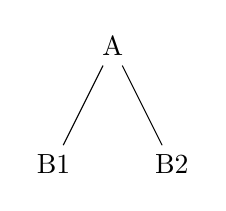
\begin{tikzpicture}
\node {A}
child{node {B1}}
child{node {B2}}
;
\end{tikzpicture}
\end{Verbatim}
      \end{minipage} gives  \hspace{2cm}
      \begin{minipage}{.35\linewidth}
        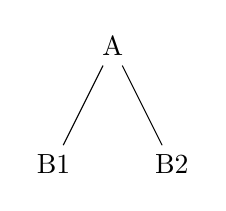
\begin{tikzpicture}
          \node {A}
            child{node {B1}}
            child{node {B2}}
          ;
        \end{tikzpicture}
      \end{minipage}
    \item Grids: use \verb|\draw[<options>] (a) grid (b)| where \texttt{(a)} and \texttt{(b)} are the endpoint of a diagonal (we assume a rectangular mesh). Options may include \texttt{step=<n>}, which sets the width of the cells. The options \texttt{xstep} and \texttt{ystep} are available, as well.
    \item Arrows - heads: \href{https://gist.github.com/AndiH/f99d9b0cbd3519c27af5b96cfbeff97c}{list}, customization \href{https://tex.stackexchange.com/questions/5461/is-it-possible-to-change-the-size-of-an-arrowhead-in-tikz-pgf/161238#161238}{here}.
    \item One may want to have a look at the section about loops, \autoref{sec:loops}.
    \item ATTENTION: for big pictures it is advised to used the \texttt{TikZ} library \texttt{external} in order to avoid regenerating the picture ad each compilation.
%
  \end{itemize}
  %%%%%%%%%%%%%%%%%%%%%% pgfplots
  \subsection{\texttt{pgf(plots)}}
  \label{sub:pgfplots}
  With an \emph{abuse of notations}, here we gather both \texttt{pgf} and \texttt{pgfplots} (and related) tricks. Here is the \href{http://ctan.tetaneutral.net/graphics/pgf/contrib/pgfplots/doc/pgfplots.pdf}{manual}.

  Before going into the details, if you are familiar with \texttt{gnuplot} you may want to check the package \href{http://mirror.ibcp.fr/pub/CTAN/macros/latex/contrib/gnuplottex/gnuplottex.pdf}{\texttt{gnuplottex}} out.

  \begin{itemize}
    \item Basic math operations: compute the result of an expression \verb|\pgfmathparse{<expr>}|, retrieve it with \verb|\pgfmathresult| and use it. It is advised to store it in a variable with \verb|\pgfmathsetmacro\newmacro{\cmd}|
\begin{verbatim}
  \pgfmathparse{sqrt(4)*6}
  \pgfmathsetmacro\result{\pgfmathresult}
\end{verbatim}
    \item Basic plotting: examples in \href{run:./ex_plot.tex}{\texttt{ex\_plot.tex}}.
    \item 3D plot: \verb|\addplot3| example in \href{run:./ex_plot.tex}{\texttt{ex\_plot.tex}}
      \begin{itemize}
        \item For surface plots, use option \verb|surf| or \verb|mesh|. Watch out for the matrix-like structure that your data must have in order to be interpreted as an actual surface. In particular, blank-lines are very important and separate two rows.
      \end{itemize}
    \item Define commands, set global options: \verb|\pgfplotsset{[...]}|, usually in preamble (advice: use \verb|\pgfplotsst{compt=newest}| for compatibility with the most recent available version).
    \item External plot shape: The plot is usually square, one may prefer to stretch it, here are some options
      \begin{itemize}
        \item \verb!x|y post scale=<n>!;
        \item \verb!x|y scale=<n>!;
        \item \verb|unit vector ratio=<x_value> <y_value>| e.g. \verb|unit vector ratio=2 1| for a \texttt{x} axis two times longer than the \texttt{y} one
      \end{itemize}
    \item Change the width: \texttt{width=<n>cm}.
    \item Lines\ldots
      \begin{itemize}
        \item Styles: \texttt{solid}, \texttt{dashed}, \texttt{dotted}, \texttt{dashdotted}; two modifiers can be use in combination with the styles: \texttt{densely}, \texttt{loosely} (e.g. \texttt{densely dotted}, \texttt{loosely dashed}).
        \item Width: \texttt{ultra thin}, \texttt{very thin}, \texttt{thin}, \texttt{semithick}, \texttt{thick}, \texttt{very thick}, \texttt{ultra thick}. Or just: \verb|draw[line width=<n>cm, <...>] <...>;|
        \item {\bfseries ATTENTION:} the styles are passed to the markers as well, hence the markers may not appear well printed. When using \texttt{dashed, dotted} or similar remember to add also \verb|mark options={solid[,...]}|.
      \end{itemize}
    \item Markers\ldots
      \begin{itemize}
        \item \texttt{only marks} vs. \texttt{no markers}.
        \item \texttt{mark repeat=<n>}, filter the markers, print only every \texttt{n}.
        \item Look here above at the line style items in order to prevent weird looking markers.
        \item Use markers outside \texttt{tikz} environments: \verb|\pgfuseplotmark{<marker_code>}|; e.g. \verb|\pgfuseplotmark{square*}| (a \verb|\raisebox{<how_much>}{<what>}| may be needed). However, use \verb|\label{<label>}| and \verb|\ref{<ref>}| when possible.
      \end{itemize}
    \item \verb|draw=none|: (actually a \verb|TikZ| key) "switches off" line and marker drawing
    \item Plot style\ldots
      \begin{itemize}
        \item Smoothing a plot: \verb|\addplot[smooth[,...]]|
        \item Constant (stairs) plot: options \texttt{const}/\texttt{jump plot} and you may want to choose the position of the mark (\texttt{const plot mark mid}/\texttt{right}/\texttt{leftt})and fill (\texttt{fill=<color>}). Try also \texttt{jump plot}.
        \item \texttt{clip mode=individual}: later plots are plotted on top of preceding markers.
      \end{itemize}
    \item Legend\ldots
      \begin{itemize}
        \item Exclude plot from legend (and cycles): option \verb|forget plot|.
        \item Transparency: the legend box has by default a solid white background, hence it covers part of the canvas. E.g.
\begin{verbatim}
legend style={fill=none} % see-through
legend style={fill=white,fill opacity=0.3,draw opacity=1,%
              text opacity=1} % Custom
\end{verbatim}
        \item Font size: \verb|legend style={font={\scriptsize}}|
        \item Legend box color: \verb|legend style={draw={<color>}}| or \verb|none| for no box.
        \item Alignment: \verb!legend cell align=left|center|right!
        \item Scale: \verb|legend style={nodes={scale=0.7}}|
        \item Legend outside the plot: add \texttt{legend pos=outer north east} (only \texttt{north east} is available so far); or specify the position: \verb|legend style={at={(0.5,-0.1)},anchor=north}|, mind that the coordinates are relative to the axis line, hence those mean below the chart in the middle.
        \item More columns / horizontal growing: \verb|legend style={legend columns=<n>}| where \texttt{n} is the wished number of columns, \texttt{-1} means \emph{horizontally}. For horizontal, one can also use \texttt{transpose legend}
        \item Add lines not related to plot: first, use \verb|\addlegendimage{empty legend}|, the use \verb|\addlegendentry{<lorem>}| to fill the newly line. This could be useful for giving the legend a title. Of course the order is important.
        \item Interesting options: \texttt{reverse legend} (invert the order), \texttt{draw=none} (no legend bow)
      \end{itemize}
    \item Cycle lists. When printing more than one plot on the same canvas, if no options are given \texttt{pgfplots} will choose a line style itself in order to identify easily the plots. Those are the \texttt{cyle list}s.
      \begin{itemize}
        \item Choose the one to use by passing option \verb|cycle list name=<name>| or define directly one via \verb|cycle list|
        \item Some preloaded cycle lists are: \texttt{color}, \texttt{black white}, \texttt{mark list} (and starred version), \texttt{color list} (and starred version), \texttt{linestyles} (and starred version).
        \item Define new lists
\begin{verbatim}
\pgfplotscreateplotcyclelist{ACMilan}{%
  {color=red,solid},
  {color=black,solid},
  {color=red,dashed},
  {color=black,dashed} % <- No comma on the last
}
\end{verbatim}
        \item MIND:
          \begin{itemize}
            \item \verb|\addplot [<opt>]|: the style is entirely defined by \verb|<opt>| and \verb|<opt>| only,
            \item \verb|\addplot+[<opt>]|: \verb|<opt>| is appended to the \texttt{cycle list} option.
          \end{itemize}
      \end{itemize}
    \item Show colorbar: option \texttt{colorbar}. Yup, that was easy. Default is vertical on the right. One may choose \texttt{colorbar left}, \texttt{colorbar horizontal}.
    \item Print zero axes: have a look \href{https://tex.stackexchange.com/questions/55718/how-can-i-add-a-zero-line-to-a-plot}{here}.
    \item A couple of ides about confidence levels and errors: one is \href{https://tex.stackexchange.com/questions/185111/adding-confidence-intervals-in-pgfplots}{here} and the other \href{https://tex.stackexchange.com/questions/96954/plotting-two-time-series-with-bounds}{there}.
    \item Idea: \texttt{clickable coords} make something (dis)appear at mouse click.
    \item ATTENTION: for big pictures it is advised to used the \texttt{TikZ} library \texttt{external} in order to avoid regenerating the picture ad each compilation.
    \begin{itemize}
      \item A remark about compiling time when plotting from an external file is in the following, \verb|pgfplotstable|-related section.
    \end{itemize}
  \end{itemize}

\subsubsection{\texttt{pgfplotstable}}
\texttt{pgfplotstable} is a useful sub-package of \texttt{pgfplots} which, for example, enables you to read and plot directly data from a file if \href{http://mirrors.standaloneinstaller.com/ctan/graphics/pgf/contrib/pgfplots/doc/pgfplotstable.pdf}{\texttt{pgfplotstable}}.

In what follows, \verb|<table>| can be either the file to be read, or a macro associated to an already read table, or a hardcoded table (cf. \href{run:./ex_plot.tex}{\texttt{ex\_plot.tex}}).

Two are the main reasons to use/love \texttt{pgfplotstable}: creating plots from data using \verb|\addplot table {<table>};|, typesetting tables with \verb|\pgfplotstabletypeset{<table>}| (mind that this is a just an interface and \texttt{pgfplotstable} will only print the content in a format compatible with a \texttt{tabular} or alike environment). Examples are in \href{run:./ex_plot.tex}{\texttt{ex\_plot.tex}}.

  \begin{itemize}
    \item Global settings / style definitions: e.g. \verb|\pgfplotstableset{[...]}|
    \item Separators: options \verb|col sep=<char>,row sep=<char>| (default whitespace and newline).
    \item Ignore characters: option \verb|ignore chars=<chars>|.
    \item \verb|clear infinite|: if NaN or infinite are found, they are considered as empty cells.
    \item Bad data: select how to treat bad data: e.g. \verb!unbounded coords=jump|discard!.
    \item How to treat empty cells: \verb|empty cells with={<...>}|.
    \item Option \verb!header=true|false|has colnames!. Tell whether or not the first non-commented line should be treated as the names of the columns. \texttt{has colnames} force it even if it is number and not string.
    \item Sort\&Filter: options \verb|sort,sort key={<key>}| and also \href{https://tex.stackexchange.com/questions/66177/how-can-i-filter-select-data-from-a-table-and-plot-it}{here}.
    \item Warnings: when filtering or discarding data, one gets warnings, shush them with \texttt{filter discard warning=false}.
    \item Get cell content: For current row (replace \verb|this| with \verb|prev| for previous row or with \verb|next| for next row)
      \begin{itemize}
        \item \verb|\thisrow{<col_name>}|: get the value and use it now.
        \item \verb|\thisrow{<col_name>}{<\macro>}|: get the value and store it in the macro.
        \item If one wants to use column indexes (instead of column names): e.g. \verb|\thisrowno{<n>}| (zero-based).
        \item \verb|\pgfplotstablegetelem{<row>}{<col>}\of{<table>}|. The second argument must be a column name, if one wishes to use an index replace it with: \verb|{[index]<n>}|.
        \item \verb|\pgfplotstablegetcolumnnamebyindex{0}\of{\mytab}\to{\firstcolumn}|
      \end{itemize}
    \item Create columns: two main ways
      \begin{itemize}
        \item Online: dedicated option, the column is used directly
\begin{verbatim}
\pgfplotstabletypeset[%
  create on use/newcol/.style={create col/.<type>={[...]}]{<table>}
\end{verbatim}
        It works both with \verb|\pgfplotstabletypeset| and \verb|\addplot table|
        \item Offline: dedicated command, the columns will be added to the table and usable elsewhere
\begin{verbatim}
\pgfplotstablecreatecol{create col/.<type>={[...]}}{<table>}
\end{verbatim}
        \item Mind that if you want to perform operation on created columns (e.g. summing two new columns), the columns must be created offline (\href{run:./ex_plot.tex}{\texttt{ex\_plot.tex}}).
      \end{itemize}
    \item Ideas on columns management: \href{https://tex.stackexchange.com/questions/79150/pgfplotstable-how-to-access-column-name}{here}.
    \item Vertically concatenate two tables (only common columns are printed, only one header is printed): \verb|\pgfplotstablevertcat{\mytabone}{mytabtwo}|, then merged is stored in \verb|\mytabone|, hence print it: \verb|\pgfplotstabletypeset{\mytabone}| (\href{https://tex.stackexchange.com/questions/19877/add-rows-to-a-pgftable}{here}).
    \item Modify row \texttt{<n>}: e.g. print line before row number 4
\begin{verbatim}
\pgfplotstableset{%
  every row no 4/.style={before row={\hrule}}}
\end{verbatim}
    \item Compiling performances: reading at each time vs. \verb|\pgfplotstableread|. It may happen that one has a big (many columns and/or many rows) file to plot, possibly it should be used several times. If you are a not-too-bad developer, you'd be lead to read it once, store it in a variable and reuse it again and again, like this
\begin{Verbatim}[samepage=true]
\pgfplotstableread{file.dat}\mytable
% Repeat several times
% [...]
\addplot table {\mytable};
\end{Verbatim}
  However, as it is explained \href{https://tex.stackexchange.com/a/304734/206129}{here}, a faster solution is
\begin{Verbatim}[samepage=true]
% Repeat several times
% [...]
\addplot table {file.dat};
\end{Verbatim}
  For big files, the speed-up might be 2 (I indeed observed it) and more!
  \begin{itemize}
    \item Be also aware of \href{https://tex.stackexchange.com/questions/236398/speed-up-plotting-data-with-many-columns}{this}.
    \item For plots with a lot of data-points, using option \verb|each nth point=<n>| (\href{https://tex.stackexchange.com/a/68658/206129}{here}) may be worth it. If you think that reducing drastically your data points may deteriorate the quality of your plot, try adding option \verb|smooth|, too.
  \end{itemize}
  \end{itemize}

%%%%%%%%%%%%%%%%%%%%%%%%%%%%%%%%%%%%%%%%%%%%%%%%%%%%%%%%%%%%%%%%%%%%%%%%%%%%%%%%
%%%                   SECTION: DRAFT
%%%%%%%%%%%%%%%%%%%%%%%%%%%%%%%%%%%%%%%%%%%%%%%%%%%%%%%%%%%%%%%%%%%%%%%%%%%%%%%%
\section{Draft}
\label{sec:Draft}
\begin{itemize}
  \item The \verb!draft! option (passing it to the \verb!article! class, for example) will make visible the lines where you're exceeding the margin (little black vertical bar at the end of the line) and it will not load the figures but only reserve a place on the page (at least, you can see the layout): the compilation is faster
\begin{verbatim}
\documentclass[draft]{article}
\end{verbatim}
  \item Show all labels that you have set in pdf (useful when writing the source and you don't want to scroll to know the exact name that you chose for the equation you want to refer to): package \href{http://ctan.mines-albi.fr/macros/latex/contrib/showlabels/showlabels.pdf}{\texttt{showlabels}}.
  \begin{itemize}
    \item ATTENTION: make sure you load it after \texttt{amsmath} and alike, and after \texttt{hyperref}.
    \item Add support for a command: example
\begin{verbatim}
\showlabels{bibitem}
\showlabels{cite}
\end{verbatim}
  \end{itemize}
  \item An alternative for printing out the labels is \href{http://ctan.tetaneutral.net/macros/latex/required/tools/showkeys.pdf}{\texttt{showkeys}}.
  \item Fancy and colorful todo notes from the \href{http://tug.ctan.org/macros/latex/contrib/todonotes/todonotes.pdf}{\texttt{todonotes}} package.
  \item With \texttt{beamer}: \autoref{sec:Beamer}.
  % % Let the following be the last
  \item It could be interesting to define a command that may be set to either \texttt{draft} or \texttt{final}. Pass this command to all the packages listed just here above, hence you just need to modify this macro in order to change the setting of all the packages. E.g. mind that it goes before the class:
\begin{verbatim}
\providecommand{\DraftOrNot}%
%{draft}
{final}
\documentclass[\DraftOrNot]{article}
\end{verbatim}
  \item One may want to check the part about the large comments out: \autoref{sec:Miscellaneous}.
\end{itemize}

%%%%%%%%%%%%%%%%%%%%%%%%%%%%%%%%%%%%%%%%%%%%%%%%%%%%%%%%%%%%%%%%%%%%%%%%%%%%%%%%
%%%                   SECTION: REFERENCING & HYPERLINKS
%%%%%%%%%%%%%%%%%%%%%%%%%%%%%%%%%%%%%%%%%%%%%%%%%%%%%%%%%%%%%%%%%%%%%%%%%%%%%%%%
\section{Referencing \& Hyperlinks}
\label{sec:Referencing}
\begin{itemize}
  \item It is a good habit to follow this structure when naming a \texttt{label}: \verb|\label{type:desc}|. \texttt{type} is short for the type of element that is being named, for instance \texttt{fig} for a figure/picture, \texttt{sec} for a section, \texttt{eq} for an equation and so on. \texttt{desc} should clearly identify the element. For instance, see what was done wit the Euler equation in \autoref{sec:math}: \verb|\label{eq:euler}|.
  \item Some tips already given in \autoref{sec:math} and \autoref{sec:Items}
  \item Useful packages for referencing: \href{ftp://tug.ctan.org/pub/tex-archive/macros/latex/contrib/hyperref/doc/manual.pdf}{\texttt{hyperref}} and \href{http://ctan.mines-albi.fr/macros/latex/contrib/cleveref/cleveref.pdf}{\texttt{cleveref}}:
\begin{verbatim}
\usepackage{hyperref} % ATTENTION: to be loaded AFTER math related packages
\usepackage[noabbrev]{cleveref} % ATTENTION: to be loaded AFTER hyperref
\end{verbatim}
  \item ATTENTION: \texttt{cleveref} does not produce hyperlinks, it is just a smart reference-management tool. This option is provided only by \texttt{hyperref}.
  \item Referencing with type (that is, automatically getting \emph{section 1.1})
\begin{verbatim}
\autoref{label} % with package hyperref
\cref{label}    % with package cleveref
\end{verbatim}
  \begin{itemize}
    \item Define names for user-defined environments
\begin{verbatim}
\newcommand{\<env>autoref}{<printedenvname>} % with package hyperref
\crefname{<env>}{<singular>}{<plural>} % For cref (cleveref)
\end{verbatim}
    \item Capitalize the name (e.g. \emph{Section 1.1}): possible with \texttt{cleveref}
\begin{verbatim}
\Cref{label} % instead of cref
\end{verbatim}
          or
\begin{verbatim}
\usepackage[capitalise]{cleveref} % both \cref and \Cref capitalized
\end{verbatim}
  \end{itemize}
\item Referencing by names (and not numbers): have a look \href{https://texfaq.org/FAQ-nameref}{here}.
\end{itemize}

The \texttt{hyperref} package enables to create hyperlinks. Here is an \href{https://www.overleaf.com/learn/latex/hyperlinks}{overview} (the previous word is indeed a hyperlink! Click on it!). The basic command is \verb|\href{<link_address>}{<place_holder>}|: \verb|place_holder| is what is printed in the document and \verb|link_address| is the actual address.
\begin{itemize}
  \item Webpages: it is better to prepend \texttt{http://} (or indeed \texttt{https://}) to the link in order not to have weird behavior, e.g. \verb|https://www.edf.fr|.
  \item Email address: prepend \texttt{mailto:} to the address, e.g. \verb|\href{mailto:jbl_pdg@gmail.com}{JBL}|.
  \item Local file: prepend \texttt{run:} to the file you want to open, e.g. \verb|\href{run:/path/to/tips.pdf}{tips}|.
\end{itemize}

Some tips about \texttt{cleveref}:
\begin{itemize}
  \item \verb|\labelcref{<label>}|: print only the label. E.g. \texttt{1.1} (without \texttt{Section}).
  \item \verb|\namecref{<label>}|: print only the name, type. E.g. \texttt{Section} (without \texttt{1.1}).
  \item \verb|\crefrange{<start_label>}{<end_label>}|: typeset a range of references. For uppercase names \verb|\Crefrange{<start_label>}{<end_label>}|
  \item option \texttt{noabbrev} makes \texttt{cleveref} print full reference name, e.g. \texttt{equation} instead of \texttt{eq.}
  \item option \texttt{poorman}: you are invited to look at it in the \href{http://ctan.mines-albi.fr/macros/latex/contrib/cleveref/cleveref.pdf}{manual}. Basically, if you have to send your \TeX~sources to someone that does not use \texttt{cleveref}, you can add this option and \texttt{cleveref} will produce a \texttt{sed} script which, once run, will replace all calls to its macros although leaving the output unchanged.
\end{itemize}

%%%%%%%%%%%%%%%%%%%%%%%%%%%%%%%%%%%%%%%%%%%%%%%%%%%%%%%%%%%%%%%%%%%%%%%%%%%%%%%%
%%%                   SECTION: BIBLIOGRAPHY
%%%%%%%%%%%%%%%%%%%%%%%%%%%%%%%%%%%%%%%%%%%%%%%%%%%%%%%%%%%%%%%%%%%%%%%%%%%%%%%%
\section{Bibliography}
\label{sec:Bibliography}
\begin{itemize}
  \item \href{https://www.overleaf.com/learn/latex/Bibliography_management_with_bibtex}{Here} you can find a basic introduction to the bibliography in \LaTeX. A good habit is to create a separate \texttt{.bib} file. Some pdf managing programs (such as \href{https://www.zotero.org/}{Mendeley} or \href{https://www.zotero.org/}{Zotero}) automatically build the \texttt{.bib} file for you, with all the pdf in your library.  \item There are several ways to manage the bibliography in TeX files: \texttt{biblatex}, \texttt{natbib},\ldots
  \item Examples of bibliography styles can be found \href{https://www.overleaf.com/learn/latex/Bibtex_bibliography_styles}{here};
  \item Print references even if they were not cited: \verb|\nocite{<ref_name>}|. Print all the references: \verb|\nocite{*}|.
\end{itemize}

  \subsection{\texttt{natbib}}
  \href{https://ctan.crest.fr/tex-archive/macros/latex/contrib/natbib/natbib.pdf}{User guide} (in \href{http://mirror.ibcp.fr/pub/CTAN/info/translations/natbib/fr/f-natbib.pdf}{French} too!) and \href{http://mirror.ibcp.fr/pub/CTAN/macros/latex/contrib/natbib/natnotes.pdf}{cheat-sheet} or this \href{http://merkel.texture.rocks/Latex/natbib.php}{cheat-sheet too}. If you do not use a \LaTeX{} integrated editor (IDE) (although it could be useful to know this anyway) but compile from terminal, you should:
    \begin{enumerate}
      \item Compile one time with your preferred compiler (e.g. \texttt{pdflatex}: \verb|$pdflatex main.tex|);
      \item Compile the bibliography with \texttt{bibtex}: \verb|$bibtex main.aux|;
      \item Re-compile \textbf{twice} your \texttt{.tex} in order to have all the references linked and working.
    \end{enumerate}

    \begin{itemize}
      \item If you have more than one bibliography files, just put them in the \texttt{bibliography} command separated by a comma (remember that you should not write the extension \texttt{.bib}):
    \begin{verbatim}
      \bibliography{my_biblio_1,my_biblio_2}
    \end{verbatim}
      \item \texttt{natbib} automatically creates a new section for the references. One get rid of it by overriding the \texttt{bibsection} command: one may choose to defining it as a subsection, or simply remove it, as follows
\begin{verbatim}
  \renewcommand{\bibsection}{}
\end{verbatim}
      \item For three or more authors, \texttt{natbib} will print \emph{First\_Author et al.}. In order to print all the authors, use the starred-version of the commands: \verb|\citep*{<ref_name>}|
      \item Multiple bibliography / bibliography in each chapter: package \href{http://wiki.davidhaberthuer.ch/latex#chapterbib}{\texttt{chapterbib}} and option \texttt{sectionbib} as explained \href{http://wiki.davidhaberthuer.ch/latex#chapterbib}{here} or \href{https://tex.stackexchange.com/questions/229846/different-bibliographies-for-each-chapter-with-shared-references}{here}. Remember to call \verb|\bibliography{<chap_bib>}| in each chapter. Another possibility is package \href{http://mirrors.standaloneinstaller.com/ctan/macros/latex/contrib/bibunits/bibunits.pdf}{\texttt{bibunits}}, have a look \href{https://texfaq.org/FAQ-chapbib}{here}.
    \end{itemize}

  \subsection{\texttt{biblatex}}
  \href{http://mirror.ibcp.fr/pub/CTAN/macros/latex/contrib/biblatex/doc/biblatex.pdf}{User guide} (in the introduction, there is a nice overview of other bibliography-related packages which could be useful). A quick \href{https://www.overleaf.com/learn/latex/Articles/Getting_started_with_BibLaTeX}{tutorial}. And a useful \href{http://tug.ctan.org/info/biblatex-cheatsheet/biblatex-cheatsheet.pdf}{cheatsheet}. \texttt{biblatex} relies on \texttt{biber}, thus the compiling sequence becomes:
    \begin{enumerate}
      \item Compile one time with your preferred compiler (e.g. \texttt{pdflatex}: \verb|$pdflatex main.tex|);
      \item Compile the bibliography with \texttt{biber}: \verb|$biber main.bcf|;
      \item Re-compile \textbf{twice} your \texttt{.tex} in order to have all the references linked and working.
    \end{enumerate}
  If you use an IDE, you may have to change the compiling stage command to something like: \verb|biber %.bcf|. However, \texttt{biber} is not available on the EDF-controlled OS, but you can change the bibliography compiler. When loading \texttt{biblatex} use \texttt{bibtex} or \texttt{bibtex8} as backend (both available on EDF PCs): e.g. \verb|\usepackage[backend=bibtex]{biblatex}|. Now the compiling process will be the same as for \texttt{natbib}:
    \begin{enumerate}
      \item Compile one time with your preferred compiler (e.g. \texttt{pdflatex}: \verb|$pdflatex main.tex|);
      \item Compile the bibliography with \texttt{bibtex}, \verb|$bibtex main.aux|, or with \texttt{bibtex8}, \verb|$bibtex8 main.aux|;
      \item Re-compile \textbf{twice} your \texttt{.tex} in order to have all the references linked and working.
    \end{enumerate}
    In IDE such as \TeX Maker, the default compiling command is usually \texttt{bibtex}, hence if you are using \texttt{bibtex8} you should modify it accordingly: \verb|bibtex8 %.aux|

  \begin{itemize}
    \item It is preferable to load \texttt{biblatex} \emph{before} \texttt{hyperref};
    \item The file containing the bibliography is set in the preamble, it is advised to do it just after you load the package:
\begin{verbatim}
  \usepackage{biblatex}
  \addbibresource{my_biblio.bib}
\end{verbatim}
    \item Print the bibliography: \verb|\printbibliography|;
    \item Set the style: use option
      \begin{itemize}
        \item \texttt{citestyle=<style>} for the \emph{citation} style (what appears when your call \verb|\cite{}|),
        \item \texttt{bibstyle=<style>} for the style in the list,
        \item \texttt{style=<style>} for setting both of the above.
      \end{itemize}
    \item Sort the citations: \verb|\usepackage[sorting=<style>]{biblatex}|, usually the argument is a combination of \texttt{n} (for name), \texttt{t} (title), \texttt{y} (year) according to the importance (e.g. \texttt{nyt}, \texttt{nty});
    \item Footnote-like citation (could be useful in \texttt{beamer}): \verb|\footcite{<ref_name>}|, look also \verb|\footfullcite{<ref_name>}|;
    \item Avoid \emph{et al.}: put in the options when loading the package \texttt{maxnames=<n>} or \texttt{minnames=<n>};
    \item No URL, ISSN, nor DOI: options \texttt{url=false,doi=false,isbn=false};
    \item Add \emph{see}, \emph{chapter n} or alike: \verb|\command[<prenote>][<postnote>]{<ref_name>}|. For example, \verb|\parencite[see][chpt 2]{Aliceetal}| gives something like: (see \emph{Alice et al.}, chpt 2)
    \item Option \texttt{backref} puts after each bibliography entry the pages/places where that entry has been cited.
    \item Avoid the warning about \texttt{utf8} encoding (possibly if the backend is set to \texttt{bibtex}): pass option \texttt{bibencoding=ascii}. However, this may cause problems if you use non-ASCII character (fancy accented symbols,\ldots).
    \item When using \texttt{biblatex} and \texttt{babel}, it is advised to load \texttt{csquotes} as well, in order to ensure that quoted texts are typeset according to the chosen language rules.
    \item Group of references:
\begin{verbatim}
\DeclareBibliographyCategory{<category}
\addtocategory{<category}{<ref_key>[,<ref_keys>]}
\end{verbatim}
      \begin{itemize}
        \item Print only/other than category: \verb|\printbibliography[[not]category=<category>]|
        \item Print only/other than type: \verb|\printbibliography[[not]type=<type>]|, with \texttt{type} being article, book\ldots
      \end{itemize}
    \item According to the style, the author in the bibliography might be replaced by a dash if it is repeated. One may disable this feature (and always print the author) with the option \texttt{dashed=false} (however, it is available only in the most recent versions ob \texttt{biblatex}: >2016)
    \item In some predefined styles, the mention "\emph{In:}" precedes the article title, for instance. One may remove it by calling: \verb|\renewbibmacro{in:}{}|. Have a look \href{https://tex.stackexchange.com/questions/10682/suppress-in-biblatex}{here} for a custom solution involving only the articles.
    \item ATTENTION: for label printing use \texttt{showkeys} (incompatibility with \texttt{showlabels} and pre/post-cite).
    \item Change size: \verb|\renewcommand{\bibfont}{\scriptsize}|
    \item Multiple bibliography / bibliography in each chapter: take advantage of the \texttt{refsegment} environment as explained \href{https://tex.stackexchange.com/questions/87414/per-chapter-bibliographies-in-biblatex}{here}. You may also want to have a look \href{https://tex.stackovernet.com/fr/q/63260}{here}.
\begin{verbatim}
  \begin{refsegment}
    \chapter{Chpt 1}
    Lorem lipsum
    \printbibliography[segment=1,title={Chpt1 references},heading=subbibintoc]
  \end{refsegment}
  \printbibliography[title={Global references},heading=subbibintoc]
\end{verbatim}
      \begin{itemize}
        \item Remember to change the number of \texttt{segment} according to the chapter
        \item If you plan to use \verb|\include| and \verb|\includeonly| with, for instance, one file per chapter you'd better NOT put \verb|\begin{refsegment}| in the chapter \texttt{.tex} but leave it in the main, in order to avoid problem with undefined segment when \verb|\includeonly| is used
\begin{verbatim}
  \begin{refsegment}
    \include{chpt1}
  \end{refsegment}
  \printbibliography[title={Global references}, heading=subbibintoc]
\end{verbatim}
      \end{itemize}
  \end{itemize}

  Have a look at the \href{http://ctan.mines-albi.fr/macros/latex/contrib/biblatex/doc/biblatex.pdf}{here} for more details about these options/commands and many useful other ones.

%%%%%%%%%%%%%%%%%%%%%%%%%%%%%%%%%%%%%%%%%%%%%%%%%%%%%%%%%%%%%%%%%%%%%%%%%%%%%%%%
%%%                   SECTION: Standalone
%%%%%%%%%%%%%%%%%%%%%%%%%%%%%%%%%%%%%%%%%%%%%%%%%%%%%%%%%%%%%%%%%%%%%%%%%%%%%%%%
\section{\texttt{standalone}}
The standalone bundle allows users to easily place picture environments or other material in own source files and compile these on their own or as part of a main document.  A special standalone class is provided for use with such files, which by default crops the resulting output file to the content. The standalone package enables the user to simply load the standalone files using \verb|\input| inside a main document (from the \href{http://ctan.mines-albi.fr/macros/latex/contrib/standalone/standalone.pdf}{manual}). Basically one can create a file that can be compiled by itself or that can be part or a larger project, without having to change it.
\begin{itemize}
  \item A typical call would be: \verb|\documentclass[border=1mm]{standalone}|.
  \item Packages-related options: \texttt{TikZ}, \texttt{beamer}
  \item Write equations in standalone: use option \texttt{preview}.
  \item Some options:
    \begin{itemize}
      \item \verb|class=<class_name>|: set the underlying layout (article, report\dots)
      \item \verb!crop=true|false!: crop the content to its natural size plus a border
      \item \verb!multi=true|false!: if false only one big page
      \item \verb|multi={<env_name[,...]>}|: create a new page for every \verb|<env_name>| environments
      \item \verb|beamer|: crop is disabled and content shown on a blank \texttt{beamer} frame
      \item \verb|tikz|: load \texttt{TikZ} and set \verb|multi=tikzpicture|
    \end{itemize}
\end{itemize}

\textbf{Remark}: if you just want a minimal layout for a \texttt{documentclass}, an option could also be \texttt{minimal} instead of \texttt{standalone}.

%%%%%%%%%%%%%%%%%%%%%%%%%%%%%%%%%%%%%%%%%%%%%%%%%%%%%%%%%%%%%%%%%%%%%%%%%%%%%%%%
%%%                   SECTION: Thesis
%%%%%%%%%%%%%%%%%%%%%%%%%%%%%%%%%%%%%%%%%%%%%%%%%%%%%%%%%%%%%%%%%%%%%%%%%%%%%%%%
\section{Writing a thesis}
\label{sec:thesis}
A thesis is, usually, a big multi-file project. The class \texttt{book} or \texttt{memoir} is conventionally used. Here, one can find some common ideas and settings for the structure, the layout and general managing of a thesis.
\begin{itemize}
  \item Management (\texttt{include} and alike): see \autoref{sec:Sectioning}, and \href{https://en.wikibooks.org/wiki/LaTeX/Modular_Documents}{here}.
  \item The \texttt{book}-class special structure: see \autoref{sec:Sectioning}.
  \item Table of Content in each chapter: package \href{http://texdoc.net/texmf-dist/doc/latex/minitoc/minitoc.pdf}{\texttt{minitoc}}. Remark: it is built for the \texttt{book} class, it may work with \texttt{memoir} thanks to a \href{https://tex.stackexchange.com/questions/291743/minitoc-of-wrong-chapter}{workaround}.
    \begin{itemize}
      \item Problems with starred chapter* and \verb|\addcontentsline{toc}{chapter}{title}|: use instead \verb|\addchaptermtc[title]| (a less elegant option in \verb|\adjustmtc[<n>]|) as explained in this \href{https://texnique.fr/osqa/questions/5022/minitoc-un-chapitre-en-retard}{post} (in French) or in the manual. Another options is to avoid \verb|\addcontentsline| and use \verb|\addstarredchapter{<title>}|
    \end{itemize}
  \item Bibliography in each chapter: see \autoref{sec:Bibliography}. We suggest using \texttt{biblatex}, especially if you want per-chapter and global references at the same time, have a look \href{https://tex.stackexchange.com/questions/168713/global-and-per-chapter-bibliographies}{here} or \href{https://tex.stackexchange.com/questions/168713/global-and-per-chapter-bibliographies}{here}.
  \item Appendices: package \href{http://ctan.tetaneutral.net/macros/latex/contrib/appendix/appendix.pdf}{\texttt{appendix}}
    \begin{itemize}
      \item Have a look at the \texttt{toc}- and \texttt{title}-related options.
      \item For global appendices: \verb|\begin{appendices} ... \end{appendices}| and use \texttt{chapter}.
      \item For chapter appendices: \verb|\begin{subappendices} ... \end{subappendices}|. Look \href{https://tex.stackexchange.com/questions/120716/appendix-after-each-chapter}{here}.
    \end{itemize}
\end{itemize}

%%%%%%%%%%%%%%%%%%%%%%%%%%%%%%%%%%%%%%%%%%%%%%%%%%%%%%%%%%%%%%%%%%%%%%%%%%%%%%%%
%%%                   SECTION: Code & algorithms
%%%%%%%%%%%%%%%%%%%%%%%%%%%%%%%%%%%%%%%%%%%%%%%%%%%%%%%%%%%%%%%%%%%%%%%%%%%%%%%%
\section{Code \& algorithms}
\label{sec:code}
One could be lead to include a snippet, a piece of code or describe an algorithm in his \texttt{.tex}. General guidelines may be found \href{https://www.overleaf.com/learn/latex/algorithms#Listings_package}{here}, or, even better (more complete) \href{https://en.wikibooks.org/wiki/LaTeX/Algorithms}{here}. Here are some options.
\begin{itemize}
  \item \href{https://mirrors.chevalier.io/CTAN/macros/latex/contrib/listings/listings.pdf}{\texttt{listings}}: it supports code-specific syntax-highlighting, perfect if one wants to dump a snippet of code. One can even define a custom syntax-highlighting, his own language.
  \item \href{http://tug.ctan.org/macros/latex/contrib/algorithm2e/doc/algorithm2e.pdf}{\texttt{alorithm2e}}: for pseudo-code and algorithm explanation.
  \item One very basic option is to use the \texttt{verbatim} utility of \TeX~(see \autoref{sec:Miscellaneous} for some tips). It is the right choice if one has to put a couple of lines and if one does not bother with syntax-highlighting.
\end{itemize}

%%%%%%%%%%%%%%%%%%%%%%%%%%%%%%%%%%%%%%%%%%%%%%%%%%%%%%%%%%%%%%%%%%%%%%%%%%%%%%%%
%%%                   SECTION: TeXMaker
%%%%%%%%%%%%%%%%%%%%%%%%%%%%%%%%%%%%%%%%%%%%%%%%%%%%%%%%%%%%%%%%%%%%%%%%%%%%%%%%
\section{\TeX Maker}
\label{sec:texmaker}
\TeX Maker is a user-friendly IDE for creating \TeX~projects. For example, you can have both the source file and its result (i.e. the pdf) in the same windows. We should give here just some useful tips which are often unknown to the user.
\begin{itemize}
  \item {\bfseries Jump between source and pdf.} In large projects, it is often useful to go to the zone in pdf which corresponds to the line you are currently editing, for example in order to have a look at the result, or vice versa. This is easily done. First of all, ensure that you have in the \texttt{PdfLaTeX} command from the tab \texttt{Options>Configure Texmaker>Commands}, the option \texttt{-synctex=1} (it should be there by default) and compile with \texttt{pdflatex} (the easiest way is to run a \emph{Quick Build} after having checked that in corresponding tab in \texttt{Options>Configure Texmaker}, \texttt{PdfLaTeX} is selected: again, this should be the default choice). ATTENTION: this works only with the pdf viewer of Texmaker (if you open externally the pdf, for instance with \texttt{evince}, you will not be able to jump)
    \begin{itemize}
      \item From source to pdf: right click on a word then \texttt{Jump to pdf}. Shortcut: \texttt{Ctrl + Space}
      \item From pdf to source: right click on the page then \texttt{Click to jump to the line}. Shortcut: \texttt{Ctrl + click}
    \end{itemize}
  \item {\bfseries Dictionaries.} You can change the language of the spelling check by providing the selected dictionary in the related space in \texttt{Options>Configure Texmaker>Editor}. If you cannot find the desired dictionary, you should install it. First, download the dictionary: the \emph{Apache OpenOffice} / \emph{LibreOffice} extension (\texttt{.oxt}) will suffice. For example, you can find the English one \href{https://extensions.libreoffice.org/extensions/english-dictionaries}{here} or \href{https://extensions.openoffice.org/en/project/english-dictionaries-apache-openoffice}{here}. Unzip it wherever you want, provide its path in the \TeX Maker options as explained here above.
\end{itemize}

%%%%%%%%%%%%%%%%%%%%%%%%%%%%%%%%%%%%%%%%%%%%%%%%%%%%%%%%%%%%%%%%%%%%%%%%%%%%%%%%
%%%                   SECTION: latexmk
%%%%%%%%%%%%%%%%%%%%%%%%%%%%%%%%%%%%%%%%%%%%%%%%%%%%%%%%%%%%%%%%%%%%%%%%%%%%%%%%
\section{\texttt{latexmk}}
\label{sec:latexmk}

As we have seen in \autoref{sec:Referencing}, the compilation of a \LaTeX~documents involves different stages and may take some time. In fact, one has to: \begin{inparaenum}[1)] \item compile the \texttt{.tex}, \item (possibly) compile the bibliography, \item (possibly) compile the glossary, and \item the compile the \texttt{.tex} again once or twice. \end{inparaenum} \texttt{latexmk} can do this automatically by itself and it even checks if a compilation is truly needed, and, if not, it skips it. It is often shipped with the \TeX~engines (e.g. \TeX{}Live for Unix), so you may have it already. Here is the \href{http://ctan.tetaneutral.net/support/latexmk/latexmk.pdf}{manual} and a real quick \href{https://mg.readthedocs.io/latexmk.html}{tutorial}. The usage it's really simple: \verb|latexmk [<opt>] file.tex|, and that's it, it does the magic itself, all the needed compilations.

Some useful options (please refer to the \texttt{man} page for more details):
\begin{itemize}
  \item \verb|-pdf|: produce a pdf output;
  \item \verb|-g|: process regardless of file timestamps;
  \item \verb|-pdflatex=<program>|: set program used when compiling latex;
  \item \verb|-latexoption=<opt>|: add the given option to the latex command;
  \item \verb|-c|: clean the compilation files, except pdf/dvi/ps;
  \item \verb|-C|: clean also pdf/dvi/ps;
  \item \verb|-pv|: show preview;
  \item \verb|-pvc|: preview and continuously update (!!!);
\end{itemize}

Configuration and default parameters can be added to a \texttt{.latexmkrc} file. There can be several of them, in your home and in the project directory: all of them will be read, the one the project directory prevails. For instance, one can put in the \texttt{.latexmkrc}:
\begin{itemize}
  \item Add extension of generated file that should cleaned: \verb|push @generated_exts, "synctex.gz";|
  \item Set pdf command: \verb|$pdflatex = 'pdflatex -file-line-error -interaction=nonstopmode';|
  \item Set pdf viewer: \verb|$pdf_previewer = 'start evince';|
  \item Set pdf compilation chain: \verb|$pdf_mode = 1;| with
    \begin{itemize}
      \item \texttt{1}: tex to pdf,
      \item \texttt{2}: tex to ps to pdf;
    \end{itemize}
  \item Set bibliography treatment: \verb|$bibtex = 0;| with
    \begin{itemize}
      \item \texttt{0}: never run \texttt{bibtex}/\texttt{biber};
      \item \texttt{1}: if the source file needs \texttt{.bbl}, run \texttt{bibtex}/\texttt{biber} only if the relevant \texttt{.bib} files exists; \texttt{.bbl} are never erased in a clean-up;
      \item \texttt{1.5}: as \texttt{1} but \texttt{.bbl} are erased in a clean-up;
      \item \texttt{2}: always run \texttt{bibtex}/\texttt{biber} if needed.
    \end{itemize}
\end{itemize}

If no files are given to the command, \texttt{latexmk} will try to compile all the \texttt{.tex} that it finds, which might not be the wished output when one is working on a large projects with multiple source files. To overcome this, one can set one or more main files in the local \texttt{.latexmkrc}:
\begin{verbatim}
  @default_files = ('main.tex'[,'maint_2.tex'...]);
\end{verbatim}
One is also advised to put the following piece of code in the first line of a dependent \texttt{.tex}, hence pointing to the main file:
\begin{verbatim}
%! TEX root = path/to/main.tex
\end{verbatim}

%%%%%%%%%%%%%%%%%%%%%%%%%%%%%%%%%%%%%%%%%%%%%%%%%%%%%%%%%%%%%%%%%%%%%%%%%%%%%%%%
%%%                   SECTION: Loops
%%%%%%%%%%%%%%%%%%%%%%%%%%%%%%%%%%%%%%%%%%%%%%%%%%%%%%%%%%%%%%%%%%%%%%%%%%%%%%%%
\section{Loops}
\label{sec:loops}
  \begin{itemize}
    \item Load \verb|pgffor| (it is already loaded by \verb|TikZ| and by the \verb|pgf*| packages, cf. \autoref{sec:tikzpgf}).
    \item A quick \href{https://stuff.mit.edu/afs/athena/contrib/tex-contrib/beamer/pgf-1.01/doc/generic/pgf/version-for-tex4ht/en/pgfmanualse15.html}{guide}.
    \item Structure:
\begin{verbatim}
\foreach <variables> in {<list>} {<commands>}
\end{verbatim}
    \item Hands-on start:
\begin{Verbatim}[samepage=true]
\foreach \what in {apple,banana,cinnamonbun}{
  I eat a yellow~\what. \\ % ~ = force space, one never knows
}
\end{Verbatim}
      one may choose to name the for-loop variable \verb|\what| as he wishes.
    \item Two variables:
\begin{Verbatim}[samepage=true]
\foreach \what\color in {apple/red,banana/yellow,cinnamonbun/creamy}{
  I eat a \color~\what. \\
}
\end{Verbatim}
    \item Let's nest them:
\begin{Verbatim}[samepage=true]
\foreach \what in {apple,banana,cinnamonbun}{
  \foreach \color in {red,yellow,creamy}{
    I eat a \color~\what. \\
  }
}
\end{Verbatim}
    \item \LaTeX~understands the argument of the list. Examples
      \begin{itemize}
        \item \verb|{1,2,...,6}| yields \verb|{1,2,3,4,5,6}|
        \item \verb|{10,9,...,0}| yields \verb|{10,9,8,7,6,5,4,3,2,1,0}| (Happy new year!)
        \item \verb|{1,3,...,7}| yields \verb|{1,3,5,7}|
        \item \verb|{1,2,...,6,a,b,...,e}| yields \verb|{1,2,3,4,5,6,a,b,c,d,e}|
        \item \verb|{1.25,1.50,...,2}| yields \verb|{1.25,1.50,1.75,2.00}|
        \item and so on
      \end{itemize}
    \item \verb|\breakforeach| breaks the loop, quits it (that was easy, wasn't it?).
    \item If the variables are to be used in \verb|pgfplots*| (\autoref{sub:pgfplots}) commands, it is better to use \verb|pgfplotsinvokeforeach| which has a slightly different structure. Here is an example. Notice that one denotes the variables as one would in a \verb|\newcommand|-like framework, with an \#
\begin{Verbatim}[samepage=true]
\pgfplotsinvokeforeach{red,cyan}{%
  \addplot[color=#1] table[x=x,y=y] {mytab.dat};
}
\end{Verbatim}
  \end{itemize}

%%%%%%%%%%%%%%%%%%%%%%%%%%%%%%%%%%%%%%%%%%%%%%%%%%%%%%%%%%%%%%%%%%%%%%%%%%%%%%%%
%%%                   SECTION: MISCELLANEOUS
%%%%%%%%%%%%%%%%%%%%%%%%%%%%%%%%%%%%%%%%%%%%%%%%%%%%%%%%%%%%%%%%%%%%%%%%%%%%%%%%
\section{Miscellaneous}
\label{sec:Miscellaneous}
\begin{itemize}
  \item \href{http://pgfplots.sourceforge.net/TeX-programming-notes.pdf}{Notes} on programming with \TeX. Package \href{http://texdoc.net/texmf-dist/doc/latex/l3kernel/expl3.pdf}{\texttt{expl3}} might be interesting as well.
  \item Define \verb!\abstractname! (unless not defined by default) in English if the \verb!babel! package is used. It has to be done for every language used in the text
\begin{verbatim}
\addto\captionsenglish{
  \renewcommand{\abstractname}{<abstract_name>}%
  %\renewcommand{\abstractname}{\vspace{-\baselineskip}}% No name
}
\end{verbatim}
  \item \verb!verbatim! (print exactly the argument, no code interpretation): any character can be used as delimiter
\begin{verbatim}
\verb|\<cmd>|, \verb!\<cmd>!, ...
\end{verbatim}
  \begin{itemize}
    \item Package \href{http://ctan.mines-albi.fr/macros/latex/contrib/fancyvrb/doc/fancyvrb-doc.pdf}{\texttt{fancyvrb}}:
      \begin{itemize}
        \item show spaces (mind also the default command \verb|\textvisiblespace| which produces \textvisiblespace)
\begin{verbatim}
\begin{Verbatim}[showspaces=true]
Let us write some interspaces
\end{Verbatim}
\end{verbatim}
\begin{Verbatim}[showspaces=true]
Let us write some interspaces
\end{Verbatim}
    \item Use \texttt{verbatim} in titles or with \texttt{hyperref}-related macros: \verb!\Verb|<cmd>|! macros:
\begin{verbatim}
\section{The 1001 advantages of \protect\Verb|fancyvrb|}
\end{verbatim}
    \item Keep it on the same page: option \verb|samepage=true|
    \item It can do line-numbering, framed boxes, select lines to print, erase characters, allow color, define escape characters\ldots
\end{itemize}
  \end{itemize}
  \item Math symbols in titles: \texttt{hyperref} usually gives a warning or even an error. Use:
\begin{verbatim}
\texorpdfstring{$ \alpha $}{alpha}
\end{verbatim}
  \item Checkmark and Xmark
\begin{verbatim}
\usepackage{pifont}
\newcommand{\cmark}{\ding{51}} % Checkmark; Try also 52
\newcommand{\xmark}{\ding{55}} % Xkmark; Try also 56
\end{verbatim}
  \item Dummy text
\begin{verbatim}
\usepackage{lispum}
%[...]
\lipsum[<paragraph>]
\end{verbatim}
  \item Deal with \verb!No room for a new [...]!-style errors: \verb|\usepackage{etex}|
  \item Framed boxes: use package \href{http://mirror.ibcp.fr/pub/CTAN/macros/latex/contrib/tcolorbox/tcolorbox.pdf}{\texttt{tcolorbox}} or \href{https://mirrors.chevalier.io/CTAN/macros/latex/contrib/mdframed/mdframed.pdf}{\texttt{mdframed}}
  \item Include external pdf: \href{http://ctan.tetaneutral.net/macros/latex/contrib/pdfpages/pdfpages.pdf}{\texttt{pdfpages}} and \verb|\includepdf{my.pdf}|, have a look \href{https://stackoverflow.com/questions/2739159/inserting-a-pdf-file-in-latex}{here}.
    \begin{itemize}
      \item With beamer \autoref{sec:Beamer}, things are a bit trickier: reset the background canvas then include your pdf.
\begin{verbatim}
\setbeamercolor{background canvas}{bg=}
\includepdf{my.pdf}
\end{verbatim}
    \end{itemize}
  \item \texttt{minipage} alignment: for multiple \texttt{minipage} on the same line
    \begin{itemize}
      \item horizontal: remember to put all of them in a \texttt{center} environment and use \verb|\hfill| between each other, so that they do not stick to the left. It is also important to \textbf{NOT} leave blank lines between them if you want them on the same line: for readability, use commented blank lines \verb|% A blank line|
      \item vertical, three options are available: \texttt{t}, vertically centered; \texttt{T}, top aligned; \texttt{b}, bottom aligned.
      \item If vertical alignment still does not work with \texttt{t}, even with other environments, such as \texttt{subfigure}, one may want to add \verb|\vskip 0pt| two the very begging of each sub-environment.
    \end{itemize}
  \item Silence warnings or errors (I discourage it, but sometimes, we get warnings for nothing): use package \href{http://ctan.mines-albi.fr/macros/latex/contrib/silence/silence-doc.pdf}{\texttt{silence}} and the command \verb|\WarningFilter[<family>]{<pacakge>}{<message>}| or \verb|\ErrorFilter| with the same arguments.
  \item Create files from \LaTeX~on-the-fly: package \href{https://mirrors.chevalier.io/CTAN/macros/latex/contrib/filecontents/filecontents.pdf}{\texttt{filecontents}}
\begin{verbatim}
\begin{filecontents}{file_name.ext}
  The content of the file
\end{filecontents}
\end{verbatim}
  \item Position of float: this is slippery ground. In theory, \LaTeX~has an algorithm that computes where it's better to print out a float (a float being something a \texttt{figure} or \texttt{table} environments), however it sometimes does a bad job and one would like to choose. Well, this is not always possible but one can make an attempt.
    \begin{itemize}
      \item First, one can tell \LaTeX~ where he prefers to have the float printed. For instance one can pass the following options (e.g. \verb|\begin{table}[<opt>]|): \texttt{h} (for \emph{here} or as close as possible), \texttt{t} (for \emph{at the top} of a page), \texttt{b} (for \emph{at the bottom} of a page), \texttt{p} (in \emph{page} of floats only, no text), \texttt{!} (to override the \LaTeX~algorithm), \texttt{H} (from package \texttt{float}, to force the position exactly \emph{Here}). Indeed, lists in order of preference are accepted: hence, \texttt{htb} means "try to print it here, otherwise at the top of a page, otherwise at the bottom of a page".
        \item Sometimes it is not enough. Clearing a page, \verb|\clearpage| or \verb|\cleardoublepage|, usually force to print all the hanging floats, so that, for example, floats form a chapter are found far and in another chapter. This kind of commands are thought for the end of a chapter or of a section, but one can also use \verb|\FloatBarrier| (from the package \href{http://mirror.ibcp.fr/pub/CTAN/macros/latex/contrib/placeins/placeins-doc.pdf}{\texttt{placeins}}) that tells \LaTeX~to print all the hanging floats before trespassing the barrier.
    \end{itemize}
  \item Captions \& co: suggested \href{https://mirrors.chevalier.io/CTAN/macros/latex/contrib/caption/caption-eng.pdf}{\texttt{caption}} package
    \begin{itemize}
      \item Change caption names, separators: well-detailed \href{https://tex.stackexchange.com/questions/17489/change-caption-name-of-figures}{post} (mind the with or without \texttt{babel} difference, related info also in \autoref{sec:languages}).
      \item Caption width: sometimes one would like to choose the caption width, for global effect pass option \verb|width=<len>| when loading \texttt{caption}, for local (only in the environment where it will be placed) \verb|\captionsetup{width=<len>}|.
    \end{itemize}
  \item \verb|\hphantom{<aaaa>}| and \verb|\vphantom<TMWpqgy>|: create a box with the width (resp. the height) of the argument and zero height (resp. width) (it basically tells \LaTeX~to reserve a horizontal or vertical space for the argument which, however, won't be printed).
  \item Get the width of an object: define a new length \verb|\newlength{\mylength}| and assign the width to it \verb|\settowidth{\mylength}{\texbf{An example}}|.
  \item \LaTeX and \verb|shell| - run some commands from inside a \texttt{.tex} and use the output. The \href{https://ctan.mc1.root.project-creative.net/macros/latex/contrib/bashful/bashful.pdf}{\texttt{bashful}} package may be useful. Also look \href{https://tex.stackexchange.com/questions/16790/write18-capturing-shell-script-output-as-command-variable}{here}. The main idea is the use of \verb|\write18|, some details \href{https://tex.stackexchange.com/questions/311084/how-to-run-shell-command-with-write18}{here}. For this kind of work, usually one should add the flag \verb|-shell-escape| to the compilation command.
  \item Package \href{https://tex.stackexchange.com/a/184075}{\texttt{environ}}: allows a more convenient definition of environments with macro \verb|\NewEnviron| (and its companion macro \verb|\BODY|)
  \item Horizontal / landscape pages
    \begin{itemize}
      \item For the whole document: use option \texttt{landscape} \verb|\usepackage[landscape]{geometry}| or \verb|\documentclass[landscape]{<class>}|.
      \item For a certain part only: have a look \href{https://tex.stackexchange.com/questions/337/how-to-change-certain-pages-into-landscape-portrait-mode}{here}. The environment is only one \verb|\begin{landscape}|, but it could come from two packages. If you are producing a pdf, use package \texttt{pdflscape} (it gives more metadata to the document that improve its readability), otherwise \texttt{lscape}.
        \begin{itemize}
          \item For horizontal numbering as well, see \href{https://tex.stackexchange.com/questions/9071/how-to-translate-and-rotate-the-heading-of-landscaped-pages}{this}.
        \end{itemize}
    \end{itemize}
  \item Conditionals
    \begin{itemize}
      \item With plain \TeX, one can define, set and use boolean as follows:
\begin{verbatim}
\newif\if<my_bool>
\<my_bool>true|false
\if<my_bool>
  [...]
\else
  [...]
\fi
\end{verbatim}
      \item Or use the \href{http://ctan.mines-albi.fr/macros/latex/base/ifthen.pdf}{\texttt{ifthen}} package, which is compatible with the plain \TeX~syntax. E.g.
\begin{verbatim}
\newboolean{<my_bool>}
\setboolean{<my_bool>}{true|false}
\ifthenelse{<conditional_statement>}
            {<if commands>}
            {<else commands>}
\boolean{<my_bool>} % Returns the truth value
\end{verbatim}
      \verb|conditional_statement| is an expression involving booleans and it can be constructed also using \verb|\AND|, \verb|\OR|, \verb|\NOT|, \verb|\([...]\)|.
    \end{itemize}
  \item For hundreds of logos (even well-known ones as Google, FB,\ldots) use package \href{https://ctan.crest.fr/tex-archive/fonts/fontawesome/doc/fontawesome.pdf}{\texttt{fontawesome}}.
  \item For typesetting units the reference package is \href{http://mirror.ibcp.fr/pub/CTAN/macros/latex/contrib/siunitx/siunitx.pdf}{\texttt{siunitx}} and its \verb|\si{<unit>}| and \verb|SI{<num>}{<unit>}| commands.
  \item Comment large parts of the file out: check this \href{https://tex.stackexchange.com/questions/17816/commenting-out-large-sections}{question}. The proposed solutions are \verb|\iffalse ... \fi|, package \href{http://mirrors.ircam.fr/pub/CTAN/macros/latex/contrib/comment/comment.pdf}{\texttt{comment}} or restructuring the project and working with \verb|\includeonly{...}|

\end{itemize}

\end{document}

